\documentclass[hidelinks,a4paper,12pt,twoside,openright]{report}
\usepackage{mystyle}

%----------------------------------------------------------------%
\makenoidxglossaries
\newacronym{slam}{SLAM}{Simultaneous Localization and Mapping}
\newacronym{imu}{IMU}{Inertial Measurement Unit}
\newacronym{gps}{GPS}{Global Positioning System}
\newacronym{ekf}{EKF}{Extended Kalman Filter}
\newacronym{icp}{ICP}{Iterative Closest Point}
\newacronym{ndt}{NDT}{Normal Distribution Transform}
\newacronym{lidar}{LIDAR}{Light Detection and Ranging}
\newacronym{radar}{RADAR}{Radio Detection and Ranging}
\newacronym{mems}{MEMS}{Micro-Electro-Mechanical Systems}
\newacronym{dof}{DoF}{Degree of Freedom}
\newacronym{pdf}{PDF}{Probability Density Function}
\newacronym{ros}{ROS}{Robot Operating System}
\newacronym{pcl}{PCL}{Point Cloud Library}
\newacronym{utm}{UTM}{Universal Transverse Mercator}
\newacronym{kitti}{KITTI}{Karlsruhe Institute of Technology and Toyota Technological Institute}

\begin{document}
\title{
\textsc{University of Bremen}\\
\vspace{15pt}
\textbf{\large MASTER'S THESIS}\\
\vspace{5pt}
\large FB1 Physics and Electrical Engineering \\
\vspace{5pt}
{\LARGE \textbf{Implementation and Evaluation of Localization Methods for Autonomous Cars}\\
\large by\\ Kerim Yener \textsc{Yurtdas}}
\vspace{2cm}
\\
\begin{tabular}{l l}
    \textbf{Examiner:} &Prof. Dr-Ing. Walter \textsc{Lang} \\
                       &Prof. Dr. Dr. h.c. Frank \textsc{Kirchner} 
\vspace{2cm}
\\
\textbf{Tutor:}        &M.Sc. Mehmed \textsc{Yueksel}\\
                       &Dr-Ing. Christoph \textsc{Hertzberg}
\vspace{4cm}
\\
                       &September 20, 2018
\end{tabular}
\vfill
\centering

\includegraphics[scale=0.06]{unib}}
%----------------------------------------------------------------%
\date{}
\author{}
\maketitle

\pagenumbering{roman}
\section*{Declaration of honour} 

I hereby confirm on my honour that I personally prepared the present academic 
work and carried out myself the activities directly involved with it. I also 
confirm that I have used no resources other than those declared. All formulations 
and concepts adopted literally or in their essential content from printed, unprinted 
or Internet sources have been cited according to the rules for academic work and 
identified by means of footnotes or other precise indications of source.
\\
The support provided during the work, including significant assistance from my
supervisor has been indicated in full.
\\
The academic work has not been submitted to any other examination authority. 
The work is submitted in printed and electronic form. I confirm that the
content of the digital version is completely identical to that of the printed version.\\
\\
Date:\line(5,0){100} \hfill Signature:\line(5,0){150}
\section*{Declaration of publication}
\begin{itemize}
\item[$\square$]I hereby agree, that my thesis will be available for third party review in
purpose of academic research.
\item[$\square$]I hereby agree, that my thesis will be available after 30 years ( § 7 Abs. 2
BremArchivG) in the university archive for third party review in purpose
of academic research.
\item[$\square$]I hereby do not agree, that my thesis will be available for third party
review in purpose of academic research.
\end{itemize}
Date:\line(5,0){100} \hfill Signature:\line(5,0){150}
\section*{Abstract}
\addcontentsline{toc}{section}{Abstract}

\section*{Acknowledgement}
\addcontentsline{toc}{section}{Acknowledgement}

\tableofcontents
\chapter*{Acronyms}
\begin{acronym}[MVVLA]
\acro{SLAM}{Simultaneous Localization and Mapping}
\acro{IMU}{Inertial Measurement Unit}
\acro{GPS}{Global Positioning System}
\acro{EKF}{Extended Kalman Filter}
\acro{ICP}{Iterative Closest Point}
\acro{NDT}{Normal Distribution Transform}
\acro{LIDAR}{Light Detection and Ranging}
\acro{RADAR}{Radio Detection and Ranging}
\acro{RMSE}{Root Mean Square Error}
\acro{MEMS}{Micro-Electro-Mechanical Systems}
\acro{DoF}{Degree of Freedom}
\acro{PDF}{Probability Density Function}
\acro{ROS}{Robot Operating System}
\acro{PCL}{Point Cloud Library}
\acro{UTM}{Universal Transverse Mercator}
\acro{KITTI}{Karlsruhe Institute of Technology and Toyota Technological Institute}
\end{acronym}
\listoffigures
\listoftables





%------------------design Header and Footer----------------------
\pagestyle{fancy}
\renewcommand{\chaptermark}[1]{\markboth{\chaptertitlename \hspace{1pt} \thechapter. #1}{}}
\renewcommand{\sectionmark}[1]{\markright{\thesection\ #1}}
\fancyhf{}
\fancyhead[LE,RO]{\textbf{\thepage}}
\fancyhead[LO]{\textbf{\rightmark}}
\fancyhead[RE]{\textbf{\leftmark}}
\fancypagestyle{plain}{%
\fancyhead{} % get rid of headers
\fancyfoot[C]{\textbf{\thepage}}
\renewcommand{\headrulewidth}{0pt} % and the line

}
%----------------------------------------------------------------%


%-------------------------------CHAPTER1-------------------------%


\chapter{Introduction}
\pagenumbering{arabic}
Throughout history, humans have consistently evolved by developing new technologies. Hence, society’s expectations for technology are continually increasing, especially expectations for automation technology, which enables a system or process to operate itself without human intervention \cite{intro_auto}. Automation technology has grown in the past few decades and has gained significant attention. It has grown especially rapidly in the field of mobile
robotics, as it underlies applications such as self-driving cars. Self-driving cars have
captured the attention of many researchers due to their wide range of applications across different fields, such as transportation, logistics, and military \cite{ACs}. Moreover, when self-driving cars reach top-level autonomy, they may save lives by preventing traffic accidents \cite{ACs1}.
\par The autonomy level of self-driving car is ranked by experts on a scale of 0–5 (see figure \ref{fig:autolevel}); level is determined by the extent to which the car can take control from the driver \cite{SAE}. As the autonomy level rises, so does exploitation of localization information, which correspondingly enhances driving safety. In many cases of autonomous driving, the vehicle needs to know where it is to execute a nontrivial task \cite{ACs2}. Therefore, localization is an essential process of autonomy and is required for levels 4 and 5 of autonomous driving.
\begin{figure}[H]
    \centering
    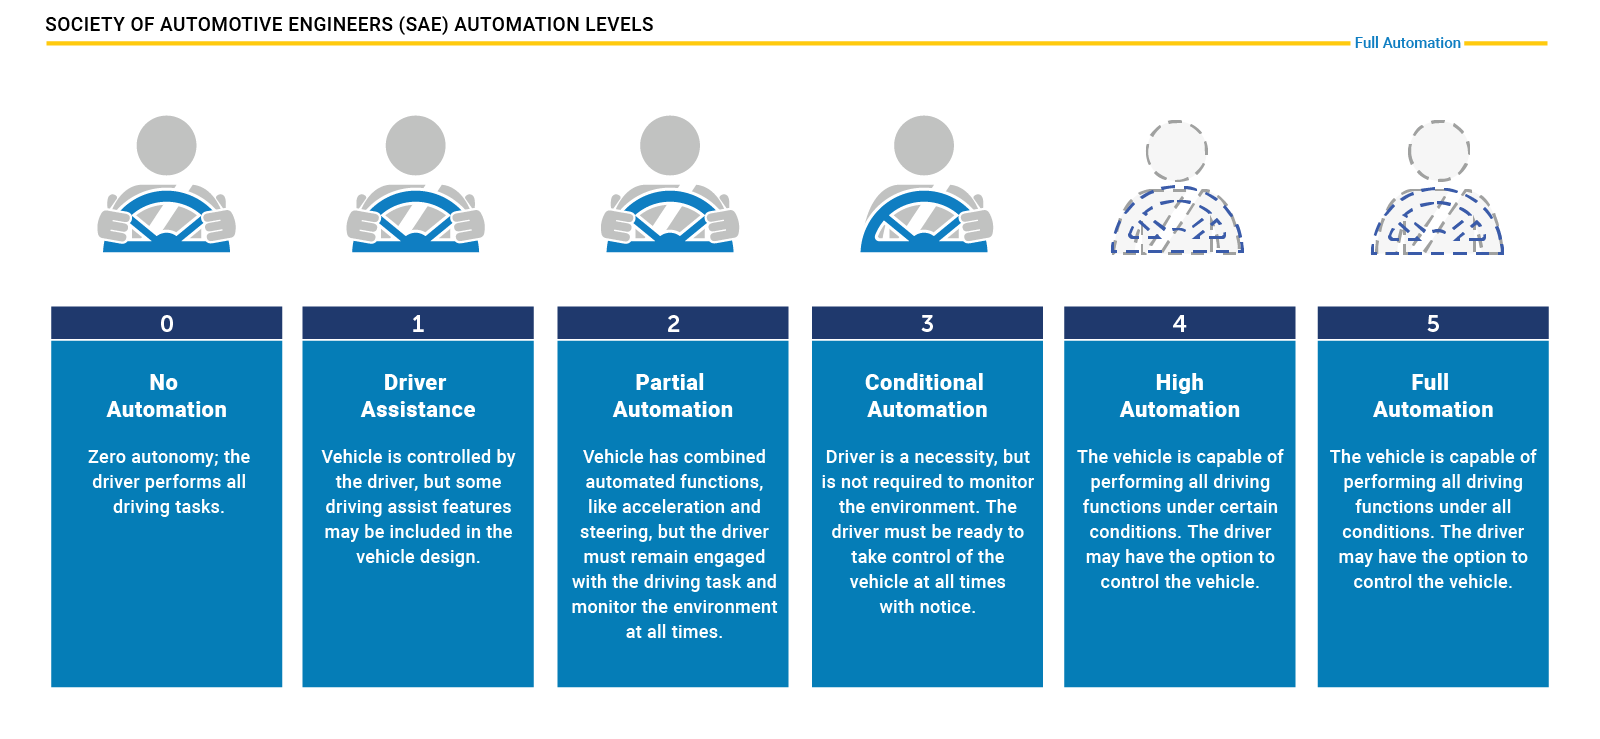
\includegraphics[scale=0.25]{autonomy_level}
    \caption{Five Levels of Vehicle Autonomy}
    \label{fig:autolevel}
\end{figure}

\par The localization problem has recently arisen in mobile robotics, and it is a hot topic addressed by many researchers. They have studied different aspect of localization ranging from low-level techniques, such as wheel odometry and dead reckoning \cite{ACs3,ACs4} to high-level techniques like map-based localization in \cite{ACs2} or \acrfull{slam} in \cite{6D_SLAM,NDT_SLAM}. Following this research, self-driving cars have continued to evolve by employing significant amounts of hardware and software that are not used in ordinary cars. For example, they use several sensors (e.g., \acrfull{lidar} and \acrfull{radar}) to perceive the environment and make decisions about vehicle control with intelligent programs.

\section{Motivation}
\par For the purpose of researching autonomous mobility, there is a vehicle platform, which is called MIAcar, have been developed under CERMcity project at  German Research Center for Artificial Intelligence (DFKI) GmbH. Since the ultimate goal of this project is to enable autonomous driving, especially in urban place, localization becomes one of the most important problem needs to be solved. At first glance, usage of the \acrfull{gps} seems to make the localization problem trivial, but in 2004 DARPA Urban Challange \cite{chp2.4}, it has been shown that GPS by itself was not able to fulfill the requirement of the competition. Moreover, it also caused to drive the vehicle off the road. Therefore, it can be easily said that localization problem still exists and it needs to be overcome by a comprehensive solution. Of note, it is important to highlight that the goal of this thesis is not beat any existing approach, instead thoroughly find most optimal localization approach for our project.
\par Taking these into consideration, this thesis aims to discuss different localization techniques, especially map-based techniques, and to address the following questions:
\begin{itemize}
    \item What kind of sensors can be used for self-driving cars?
    \item What techniques may solve the localization problem?
    \item Which methods can provide a precise localization in decimeter accuracy?
    \item Does the method work in real time on a real system? 
\end{itemize}

\section{Goal of the Master's Thesis}\label{goal}
\par The prime goals of this thesis are defined as follows:
\begin{itemize}
    \item Make a research for sensors and localization methods which are commonly used in respect of self-driving car.
    \item Analysis of different localization methods with different sensor configurations.
    \item Apply different localization methods both on simulation and real system in order to evaluate their results in terms of translation and rotation error.
    \item Allow the MIA car (see figure \ref{fig:mia1}) to perceive its environment by provided localization ability for the purpose of autonomous driving.
\end{itemize} 
\par Ideally, our study’s contribution is to demonstrate that localization methods work both theoretically and practically by improving an optimal localization method that is reliable for executing self-driving car control tasks and can be applied in a real system.
\\
\begin{figure}[H]
    \centering
    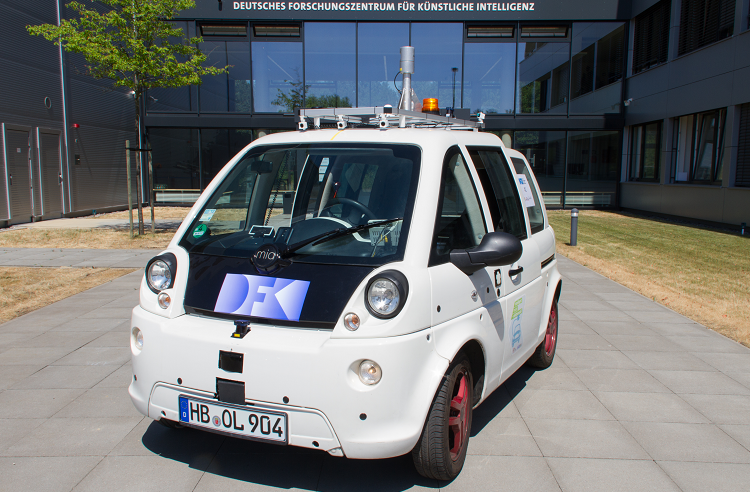
\includegraphics[scale=0.35]{mia1}
    \caption{MIAcar}
    \label{fig:mia1}
\end{figure}
\section{Thesis Organization}
The structure of the thesis is as follows:\\
\\
\textbf{Chapter \ref{chp:2}} describes different sensors and approaches for autonomous cars can be used to provide accurate localization.\\
\\
\textbf{Chapter \ref{chp:3}} covers some algorithms for estimating position of the vehicle in different aspect by using different sensor data.\\
\\
\textbf{Chapter \ref{chp:4}} describes applications of the algorithms from chapter 3.\\
\\
\textbf{Chapter \ref{chp:5}}  presents a quantitative and qualitative comparison of localization algorithms and experimental results.\\
\\
\textbf{Chapter \ref{chp:6}}  concludes this thesis and points out to new idea for future work.
%----------------------------------------------------------------%
%-------------------------------CHAPTER2-------------------------%
\chapter{State of the Art}\label{chp:2}
Centuries ago, sailors used to estimate their ships’ positions by using dead reckoning. This method relies on the ship's velocity, previous position and direction of the course in order to estimate the ship's position. At that time, a ship’s course was monitored by a magnetic compass and its velocity calculated by counting the passing knots uniformly spaced on a rope rolled out over the ship’s stern during the time a sandglass emptied  \cite{chp2.1, chp2.2}.  

\par Fortunately, there are various devices and different methods to help to estimate a vehicle's position. For this purpose, there are numerous works are presented in the literature such as different localization techniques with different sensor configuration, data fusion methodologies to find the best estimation and so forth \cite{chp2.3}. 
\par In this chapter, it focuses on the localization of self-driving cars related with the state of the art to become familiar with the concept and discuss possible different sensors and approaches which are used for the localization purpose.

\section{Sensors in Mobile Robotics}
Sensors are key devices for self-driving cars, which enables the vehicle to navigate autonomously in order to accomplish the given tasks. For this reason, self-driving cars must be equipped with several sensors that allow the vehicle to operate themselves by estimating their position relative to their environment \cite{sensor}. Since 2000, a couple quintessential examples of self-driving car's sensor configuration have emerged. Stanley and Boss, the winners of 2005 and 2007, respectively, DARPA urban challenge they showed their vehicle setup in \cite{chp2.4, chp2.5}. Both winners used almost same sensor configuration such as LIDAR, IMU, GPS, and cameras in order to win the competition. It is also important to mention that, our car has also equipped with the similar type of sensor configuration with the winners’ cars as shown in figure \ref{fig:compare_car}.
\par In the following, it describes that what sensors commonly used in the field of autonomous driving.
\begin{figure}[H]
    \centering
    \subfloat[Boss the winner of 2007 DARPA challenge taken from \cite{chp2.5}]{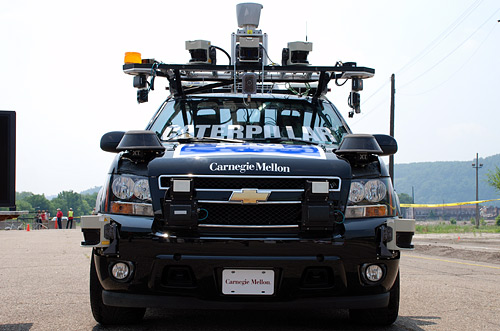
\includegraphics[scale=0.42]{boss}}
    \hfill
    \subfloat[Stanley the winner of 2005 DARPA challenge taken from \cite{chp2.4}]{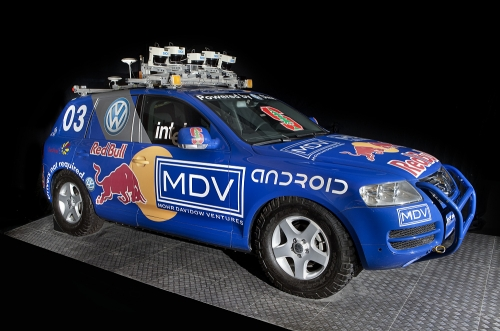
\includegraphics[scale=0.42]{stanley}}
    \caption{Two Examples for Self-driving cars}
    \label{fig:compare_car}
\end{figure}


\subsection*{Rotary encoder}

A rotary encoder is an electro-mechanical device, which reads the angular velocity of wheel in order to estimate the vehicle position \cite{chp2.6}. These sensors are used in a wide range of application even outside of the robotic field, and in most cases they are combined with either steering wheel or gyroscope to calculate wheel odometry \cite{sensor}. However, this technology has a well-known problem, that is wheel slippage \cite{odomja, odometry, odometry1}.

\subsection*{\acrfull{imu}}
\acrshort{imu} is one of the most powerful \acrfull{mems} which is used for tracking velocity and position of any dynamic object \cite{chp2.7}. Since the working principle of IMU relies on the second law of Newton, which is $F=ma$, the velocity and position of any desired object can be easily derived by taking the first and second integral of acceleration, respectively \cite{chp2.7}. Moreover, modern IMUs also provide angular velocity by means of gyroscope. However, since both gyroscope and accelerometer is prone unbounded error due to the sensor bias, therefore, IMU-based localization is subject to drift \cite{chp2.9}. Despite all these facts, IMU is one of the most commonly used sensor in self-driving cars application but it is generally combined with GPS and wheel odometry in order to increase accuracy and robustness of the localization \cite{ACs1,ACs2,chp2.4,chp2.5}.

\subsection*{\acrfull{gps}}
In many robotic application, the \acrshort{gps} is frequently used to estimate the global position of the vehicle \cite{chp2.6}. The advantage of GPS is, it can supply position information independent from the previous position and any weather conditions as long as the area is covered by satellite signals \cite{chp2.6}. However, GPS-based solution, in case of autonomous driving, can be challenging in such a place where GPS might suffer either reflection of signal or poor quality of signal \cite{chp2.10}. Therefore, it is also combined with other sensors as mentioned in \cite{chp2.4,chp2.5,kalman2,kalman6}.

\subsection*{\acrfull{lidar}}
\acrshort{lidar} is a remote sensing method which propagates a bunch of light beam to space and measures reflected light over time in order to calculate a distance of an object and determine its surface \cite{chp2.6}. Thus, LIDAR sensor enables a visualization of the surrounding environments of the vehicle in 3 dimensions in centimeter accuracy-wise. The key application of LIDAR in self-driving cars is to generate a map of an environment for purpose of path planning, obstacle detection, collision avoidance \cite{6D_SLAM,NDT_SLAM,chp2.4, chp2.5}.
\par Taken together, it is clearly understood that sensor fusion technique needs to be used in order to yield a good localization rather than using each sensor individually.

\section{Localization}
In this following sections, different localization techniques are studied as two main topics which are simultaneous localization and mapping and map-based localization.

\subsection*{\acrfull{slam}}
The concept of SLAM is that the mobile robot builds a map of its environment and meantime it estimates its position relative to the map without having any prior information \cite{slam}. 
\par Since the interest of researchers is growing in the autonomous driving field, there are lots of studies are presented to address the SLAM problem. For instance, EKF for SLAM was introduced by Cheeseman et al.\cite{slam1} whose main idea was to estimate robot pose combine with landmark position and to employ EKF to update the pose over a certain time interval. Another example is the Fast-SLAM algorithm, which was introduced by Montemerlo et al.\cite{slam2}, that is based on a particle filter. Its main focus is to deal with the non-linearity of the system whereas EKF-SLAM tries to linearize a nonlinear system which may cause the unreliability, especially for large size map, result in the solution.
\par However, due to concept of the SLAM, it is hard for self-driving cars to build map and use it concurrently for tracking their position at the same time. Therefore to simplify the SLAM problem, another approach which map-based localization (or so-called offline SLAM) is often preferred application for self-driving cars  \cite{slam3}.

\subsection*{Map-Based Localization}
The main idea of this approach is having a prior knowledge about an area for performing localization task in order to estimate and track a position of the vehicle relative to the map. For this purpose, the vehicle is driven manually around an area to acquire sensory data, in our case it was done using by LIDAR, to create map. Afterward, the map is used for localization and navigation \cite{map}. 
\par Since the map of the area is one of the requirements for map-based localization, many different methods can be used to represent the environment. The map can be created by using Graph-SLAM ,which was introduced by Lu and Milos \cite{map3}. They proposed to keep all the scan data together with defined constraint between different poses then apply least square optimization to minimize the error between poses \cite{map4}. Another example is to use scan registration (matching) methods for aligning point sets properly by calculating the transformation between two sets point \cite{icp,3dndt}. 
\par Once the map is created, different localization techniques can be applied. For instance, Monte Carlo localization (MCL) was presented by Dellart et al.\cite{map5}, which is a map based localization relies on a particle filter. An open source version of MCL available in Robot Operating System (ROS)\footnote{\url{http://wiki.ros.org/amcl}} but its application in 2D which means it is not eligible to apply for self-driving cars. Another approach is again to use scan matching methods for localization as mention in by Kato et al. \cite{map1} . They solved localization problem by matching 3D map with LIDAR scan data to find displacement between scan and map at certain time interval. The main idea of this thesis was built on these findings and modified according to the aim of this thesis "Implementation and Evaluation of Localization Methods for Autonomous Cars".


%----------------------------------------------------------------%
%-------------------------------CHAPTER3-------------------------%
\chapter{Methodology}\label{chp:3}
In this chapter, commonly used techniques for estimating robot pose according to scope of this thesis are described. In the following sections, several methods related with robot localization are explained in terms of their theoretical information, mathematical expression by considering their advantages and disadvantages. Thus, we aimed to cover some important technical background to learn how to manipulate the output of the sensors for solving the localization problem, particularly for self-driving cars.
%In this chapter, we would cover several methods which construct the outline of the thesis. Thus, we would be able to look at the localization problem from different perspectives. The main idea of this chapter is understanding the technical background and manipulating them in a way that gathering plausible information out of different sensors.
%-------------------Odometry------------------------------%
%---------------------------------------------------------%
\section{Odometry}\label{sec:odom}
To estimate a position of mobile robots there are two basic approaches: \textit{absolute} and \textit{relative positioning}. To calculate relative positioning, the odometry is used i.e., observing wheel revolutions over the time to compute traveled distance from a known starting point \cite{odometry1}. Indeed, odometry result is unreliable in a long-term due to the unbounded accumulation of error, although odometry is accepted as an essential method for robot navigation by researchers because of its attributes such as being inexpensive, straightforward and easing the fundamental problem of position determination \cite{odometry2}. 
\par Odometry employs simple geometric equations to find the displacement of the robot as follows:
\begin{equation}
    c_m = \pi D_n/nC_e \\
\end{equation}
\begin{equation}
    \Delta X_{L/R,i} = c_mN_{L/R,i} 
\end{equation}
\\
where: \\
\begin{tabular}{l l}
    $c_m$ &:coefficient that converts pulses into linear wheel displacement; \\
    $D_n$ &:wheel diameter (in cm); \\
    $n$ &:gear ratio;\\
    $C_e$ &:encoder resolution;\\
    $N_{L/R}$ &:pulse increment left and right respectively;\\
    $\Delta X_{L/R}$ &:traveled distance left and right respectively.
\end{tabular}
\newpage
\noindent The rest of the odometry equation was explained in chapter \textbf{\ref{chp:4}} in more detail. Odometry relies on above expressed equations which are easy to apply in real time on robots. However, odometry is prone to two different errors as stated by Borenstein J. et al. \cite{odometry1} these are systematic and non-systematic error. Systematic errors include unequal wheel diameters, misalignment of wheels and limited encoder sampling rate, non-systematic errors include travel over uneven grounds, travel over unexpected objects and wheel-slippage. Due to the these reasons, odometry data are not eligible to be used for a long-term as the only measure of localization.
\par Localization and its results related to wheel odometry were investigated in chapter \textbf{\ref{chp:5}} to explain these reasons in detail.
%-------------------EKF------------------------------%
%---------------------------------------------------------%
\section{Extended Kalman Filter (EKF)}\label{ekf}
As mentioned by Bordoni et D'Amico \cite{noise}, none of the sensors are perfect due to the conversion of the signal from analog to digital, therefore, sensor data are generally prone to noise. For this reason, the imperfectness should be eliminated, i.e., the noise part of the raw data must be filtered before proceeding any further application. To overcome this issue, the best approach would be Kalman filter which is introduced by Kalman R.E. (1960) \cite{kalman}. Kalman Filter is a state estimator that curtails estimated error when the requirements converge to each other \cite{kalman1}. This section is not dedicated to prove well-known Kalman filter but least understanding the concept behind it. However, its algorithm can be found in \cite{kalman}, \cite{kalman1} or \cite{kalman2}. \par Although Kalman filter is a very powerful method for estimating state, it is only defined for linear systems. Hence, Kalman filter assumes a Gaussian distribution which means Gaussian signals can keep its attribute after passing through the linear system. However, if the system is non-linear, Gaussian distribution may not be Gaussian again as shown in figure \ref{fig:Gaussion} adopted from MATLAB\footnote{\url{https://ch.mathworks.com/help/control/ref/ekf_block.html}}.
\vspace{-0,5cm}
\begin{figure}[H]
\centering
\subfloat[Linear System]{\boxed{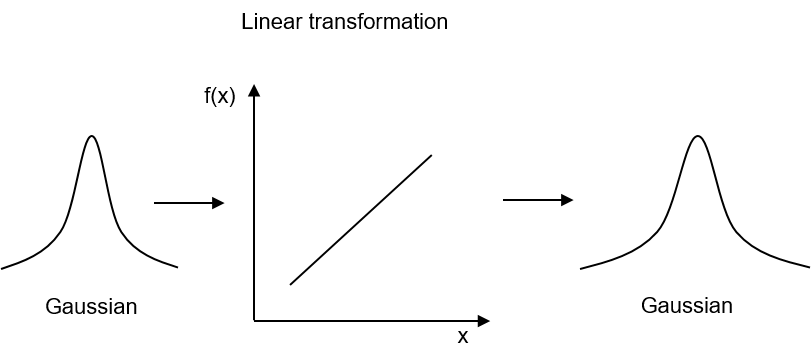
\includegraphics[height=3.9cm,width=6.5cm]{linear_new}\label{fig:linear}}}
\hfill
\subfloat[Non-Linear System]{\boxed{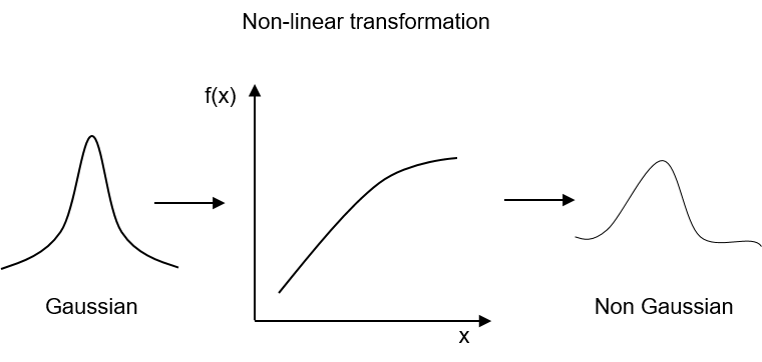
\includegraphics[height=3.9cm,width=6.5cm]{non_linear_new}\label{fig:non-linear}}}
\caption{Illustration of Gaussian over linear and non-linear system }
\label{fig:Gaussion}
\end{figure}

\par Nonetheless, from the mathematical point of view, the non-linear function can be linearized by using Taylor series expression %todo can be excluded.
that is presented by  Brook Taylor in 1715. 
Thus Kalman filter can be applied for non-linear systems as well and it is referred as \textit{extended} Kalman Filter or EKF. Let us look at the linearization of the non-linear system and set of EKF equations as stated in table \ref{tab:ekf_eq}.\\
\vspace{-1.0cm}
\begin{wrapfigure}[15]{l}{0.4\textwidth}
  \begin{center}
  \boxed{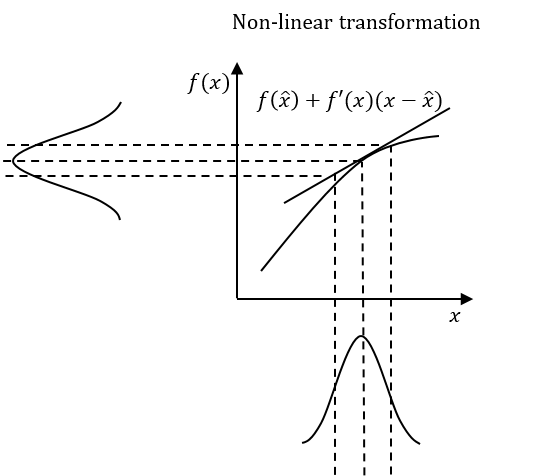
\includegraphics[width=0.4\textwidth]{linearization}}
  \end{center}
  \vspace{-18pt}
  \caption{Linearization}
  \label{fig:linearization}
\end{wrapfigure}
\vspace{10pt}
\\
\hspace{-16pt}
System:
\vspace{-20pt}
\begin{align}\label{eq:non_linear}
    &x_k=f(x_{k-1},u_k)+w_k\\
    &z_k=h(x_k)+v_k  \label{eq:non_linear1} 
\end{align}
\vspace{-10pt}
Jacobian:
\vspace{-20pt}
\begin{align}\label{eq:jacobian}
&F=\frac{\partial f}{\partial x}|_{x_{k-1},u_k}\\
&H=\frac{\partial h}{\partial x}|_{x_k}\label{eq:jacobian1}   
\end{align}
\vspace{-20pt}
Linearized:
\vspace{-6pt}
\begin{align}\label{eq:linearized}
\Delta x_k &\approx F\Delta x_{k-1} + w_k\\
\Delta z_k &\approx H\Delta x_{k} + v_k\label{eq:linearized1}
\end{align}
\\
\\
\par In equation \eqref{eq:non_linear} and \eqref{eq:non_linear1}, the non-linear system and its observation model with noise are described. Then, in the following equations \eqref{eq:jacobian} and \eqref{eq:jacobian1}, the non-linear function and its observation model are linearized by taking derivative in respect of $x$ and they are stated in equation \eqref{eq:linearized} \eqref{eq:linearized1} respectively.
\\ After the non-linear system is approximated by linearization, EKF is a good option for state estimation. Apart from its advantages, we also need to mention the disadvantages of EKF. As described by Hesam Khazraj et al. they applied EKF in respect of dynamic system estmation and they referred some of the drawbacks of EKF \cite{kalman5}. For instance, EKF is applicable as long as the higher order terms of the system are differentiable. Additionally, calculating the Jacobian matrix is also complicated and highly time-consuming. In the following, it describes how EKF is implemented on a system in general \cite{kalman4}.
\begin{table}[h]
\renewcommand{\arraystretch}{2}
    \centering
    \begin{tabular}{| c | c |}
    \hline
        \textbf{a)EKF time update equations}            &\textbf{b)EKF measurement update equations}\\
    \hline
         $x_k^-=f(\hat x_{k-1},u_k,0)$        &$\hat x_k= \hat x_k^-+K_k(z_k-h(\hat x_k^-,0))$\\
          $P_k^-=A_kP_{k-1}A_k^T+W_kQ_{k-1}W_k^T$        &$K_k=P_k^-H_k^T(H_kP_k^-H_k^T+V_kR_kV_k^T)^{-1}$\\ 
          &$P_k=(I-K_kH_k)P_k^-$\\
    \hline
    \end{tabular}
\caption{EKF equations}%todo add nice name
\label{tab:ekf_eq}
\end{table}
\subsection*{Implementation}
As a first step, one model is created for states that to be estimated as in the following equation:
\begin{equation}
     x_k = f(x_{k-1})+u_k+w_{k-1}
\end{equation}
where $x_k$ is the states of interest, $u_k$ is the control signal, which is not used in the sense of this project, and $w_k$ is the normal distributed process noise with co-variance $Q$. $A$ is the state transition matrix whereas $B$ is the control matrix. As a second step is defining observation model as following:
\begin{equation}
    z_k = Hx_k+v_k
\end{equation}
where $z_k$ is the observation vector at time k, $H$ is the measurement matrix and $v_k$ is the normal distributed measurement noise with co-variance $P$.
\par Ultimately, Kalman filter would find to correct estimation of states by calculating Time Update and Measurement Update as formulated in table \textbf{\ref{tab:ekf_eq}}. It is important to note that EKF can achieve better estimation as long as noise parameters $w_{k-1}$, $v_k$ and their co-variance $Q$ and $P$ approximated well. 
\par To conclude, EKF, which is introduced by Thomas Moore et al. \cite{kalman4}, was used in the scope of this thesis. The main reason for using EKF is to exploit all sensors on a system without dealing with different measurement time, delay or etc\cite{kalman6}. In other words, we must be able to acquire plausible information from sensors even if the absence of any sensors at any time.
%-------------------NDT------------------------------%
%---------------------------------------------------------%
\section{Normal Distribution Transform (NDT)}\label{sec:ndt}
This section focuses on the Normal Distribution Transform (NDT) which was introduced by Biber et al. \cite{2dndt} and its extended version to 3D by Magnusson et al. \cite{3dndt} for scan registration. Scan registration refers to find an affine transformation between two consecutive laser scan. In robotic fields, it is a commonly used method for providing accurate estimation of the odometry.%todo add reference and it is not common way actually it is relatively new
\par The main idea of NDT algorithm relies on a model surface by formulating the probability of finding a point at a certain position by means of the linear combination of normal distributions (see \cite{2dndt}, \cite{3dndt}), i.e, NDT breaks model point clouds into cells, which can be imaged a square in 2D or a box in 3D, and assigns a probability distribution to each cell. Thus NDT provides piece-wise representation about a model surface by means of Newton optimization algorithm \cite{2dndt}.
%TODO oku thesis localization
As mentioned before, the first step of the algorithm is breaking the space, that is occupied with points, into cells. Then, calculating the mean $\vec \mu$ of the point in the cell  and its co-variance matrix \textbf{C} for every single cell as follows \cite{2dndt}:
\begin{align}
    \vec \mu &= \frac{1}{n}\sum_{k=1}^n \vec x_k\\
    C &=\frac{1}{1-n}\sum_{k=1}^n(\vec{x_k}-\vec{\mu})(\vec{x_k} -\vec{\mu})^T
\end{align}
where $\vec x_k=1,2,3,...,n$ are the points are kept in the cell. 
\par The second step is modeling a probability that there is point at a certain position $\vec x$ in a cell by means of normal distribution and in the following equation, the \acrfull{pdf} is described \cite{3dndt}:
\begin{equation}
p(\vec x)=\frac{1}{2}exp(-\frac{(\vec{x}-\vec{\mu})^T\textbf{C}^{-1}(\vec{x}-\vec{\mu})}{2}),
\end{equation}
$\vec{p}$ is a vector that contains parameters to be optimized e.g. translation and rotation of the current pose. Let assume $\vec p=[\vec t | \vec r | \vec \phi ]$ where $\vec{t}=[t_x t_y t_z]$ is a translation, $\vec{r}=[r_x r_y r_z]$ is a rotation and $\phi$ is rotation angle. Furthermore, transformation matrix can be described by using $\vec{p}$, $\vec{x}$ and right-handed coordinate in 3D as follows \cite{3dndt}:
\\
\\
\begin{equation}
T(\vec{p},\vec{x})=
\begin{bmatrix}
tr_x^2+c		&tr_xr_y-sr_z	&tr_xr_z+sr_y\\
tr_xr_y+sr_z	&tr_y^2+c		&tr_yr_z-sr_x\\
tr_xr_z-s		&tr_yr_z+sr_x	&tr_z^2+c
\end{bmatrix}\vec{x}+ 
\begin{bmatrix}
t_x\\
t_y\\
t_z
\end{bmatrix}
\end{equation}
\\
\\
where $t$ is $1-cos\phi$, $c$ is $cos\phi$ and $s$ is $sin\phi$.
\par Next step is measuring the fitness of transformation between reference and target scan by evaluating of the sum of PDF whose value is called as score $s(p)$ in the equation \ref{eq:score}. Afterward, the fitness score is optimized until converge to the required threshold by using the Newton optimization algorithm in the equation \ref{eq:newton_opt} unless the fitness score is good enough as defined \cite{3dndt}:
\begin{equation}\label{eq:score}
    s(\vec p)=-\sum_{k=1}^np(T(\vec{p},\vec{x}))
\end{equation}
\begin{equation}\label{eq:newton_opt}
    \textbf{H}\Delta p =-g
\end{equation}
where \textbf{H} and $\vec{g}$ are the Hessian Matrix and gradient of s. Eventually, $\Delta p$ is added to the current pose in every iteration, $\vec p \xleftarrow[]{} \vec p+\Delta p$.

\subsection*{Cell size}
Since NDT represents the space with cells which are called voxel, the voxel size has a great impact on the running time and accuracy of NDT. The consequence of selecting voxel size either too big or too small cause the object in scan be more blur, increasing the running time respectively. In chapter \ref{chp:5}, this part is discussed in greater detail.
%TODO:ADD ADVANTAGE AND DISADVANTAGE
%-------------------ICP------------------------------%
%---------------------------------------------------------%
\section{Iterative closest point (ICP)}\label{icp}
Iterative closest point (ICP) is widely used for scan registration since it was presented by Besl et al. \cite{icp}. ICP is employed to approximate the path of the car by sequentially search the common points in two sets of points in a pair-wise manner. 
%todo expalin why we used it for localization
The key idea of ICP is that if the initial transformation is known between the reference and the target scan, the rest of the correct transformation in terms of the rotation matrix \textit{\textbf{R}} and translation vector \textit{\textbf{t}}, can be calculated in closed form \cite{icp1}, i.e., ICP finds the best match by utilizing the relationship between two corresponding points of two scans e.g. in the equation \eqref{eq:icp_error}, minimizing the sum of the squared distance between two matching point in two sets of points denoting as $M=\{m_1,\dots,m_{N_m}\}$ and $D=\{d_1,\dots,d_{N_d}\}$ \cite{icp4}:
\begin{align}\label{eq:icp_error}
    E(R,t)&=\sum_{i=1}^{N_m}\sum_{j=1}^{N_d}w_{i,j} ||m_i -(Rd_j+t)||^2,
    \\
    w_{i,j}&=\begin{cases}
    1, &\text{if $m_i-T*dj \leq d_{max}$}\\
    0, &\text{else}
\end{cases}%todo explain weighting 
\end{align}
where $d_{max}$ is maximum matching threshold and $w$ is weight of the pairs. The reason behind of weighting the pairs depending on $d_{max}$ is preventing misalignment and rejecting some outlier pairs as show in Figure \ref{fig:icp1}.
\begin{figure}[H]
  \centering
  \boxed{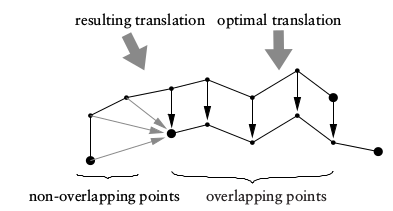
\includegraphics[scale=0.5]{icp_error.png}}
  \caption{Schematic illustration of incomplete overlap of two scans. Normal black arrows indicates corresponding point pairs whereas gray arrows indicate multi correspondences which must be eliminated for good matching. It was taken from Martin Magnusson \cite{icp2}}
  \label{fig:icp1}
\end{figure}
\vspace{-10pt}
By setting threshold ($d_{max}$) properly, the execution time would be decreased whereas the accuracy of matching would be increased. However, this is not always the case as stated in the Magnusson's study \cite{icp2} that choosing small $d_{max}$ can make ICP more susceptible so it is important to keep in mind that there is always a trade-off between time and accuracy by choosing $d_{max}$ \cite{icp3}. As a conclusion, ICP can be summarized as follows:
\begin{itemize}
    \item Determining the corresponding points in two scan
    \item Calculating rotation matrix R and translation vector t
    \item Applying a transformation to the points which is registered
    \item Iterate until fulfilling the requirement
\end{itemize}

%-------------------Summary------------------------------%
%---------------------------------------------------------%
\section{Summary}\label{sec:summary}
So far, we discussed some technical backgrounds in regard to localization of self-driving car. In the odometry part, we utilized the wheel encoder as the main sensor to estimate and track the vehicle position. Following that, we explained the EKF to facilitate synchronization of sensors such as IMU, wheel odometry, GPS and estimate the future state of the position. In the last two sections, we handled the term of scan registration in two different perspectives. Firstly, we studied NDT which is signifying the most probable points in the space as part of the surface and it does the calculation for finding the position of the vehicle in 3D point cloud depends on its assumption. In contrast, ICP is representing the surface of a model by using every single point in the space for finding the estimated pose of the vehicle. 
\par Collectively, mentioned methods above have some weakness and power, in particular, estimating the position of the vehicle. For example, wheel odometry is powerful for local localization but not for global localization due to unbounded error accumulation. EKF is useful for eliminating noises from sensors data but it is only usable when the system can be transferred into the linear system. NDT and ICP methods are capable to approximate the absolute pose of the vehicle accurately in given point cloud maps as long as initial transformation is provided. In the following chapter, their applications are studied in greater detail. 
%----------------------------------------------------------------%
%-------------------------------CHAPTER4-------------------------%
\chapter{Application}\label{app}
Now, let us have a look how this thesis was conducted after studied thoroughly the related works and the theoretical backgrounds. In following, we will first apply the odometry method by using the rotary encoder. After that, we will proceed by implementing EKF which is available in the Robot Operating System (ROS) library. In this part, we will see which parameter is used and their relation to each other. Following that, we will apply two different scan registration method which is NDT and ICP. As last thing which is the main contribution of the thesis that we will combine all these there different approaches to obtain more robust localization and fully utilize every available sensor on the system.

\section{Wheel Odometry}
Wheel odometry node\footnote{It can simply be thought an executable file in ROS package} receives the wheel displacement and steering angle information from sensors to calculate the displacement of the vehicle in a certain time slot. As consequence, the note delivers pose and velocity information in local frame as well as heading angle and its rate.
\\
\par The odomety algorithm uses the well-know kinetic equations to populates output of the node as follows.
\begin{align}
    &V_{left} = \Delta X_L*D_n/ \Delta t\\
    &V_{right} = \Delta X_R*D_n/ \Delta t\\
    &V_x = (V_{left}+V_{right})/2\\
    &R = wheelbase/sin(\alpha)\\
    &\phi = V_x * \Delta t / R\\
    &x \leftarrow x+\Delta x, \hspace{5pt} \Delta x = R * sin(\phi)\\
    &y \leftarrow y+\Delta y, \hspace{5pt} \Delta y = -(R-R*cos(\phi))
\end{align}
where $V_{left/right}$ are and velocity of left and right wheel respectively, which are calculated over elapsed time $\Delta t$. $\alpha$ is steering angle which is provided by steering wheel for calculating $\phi$ is heading angle and as a last,  position of the vehicle is estimated in direction of $x$ and $y$ in local frame by using turning radius $R$ which depends on steering angle $\alpha$ and difference between front and rear wheel $wheelbase$.\\
%we can easily derive displacement of the car over time in equation:
\begin{figure}[H]
    \begin{subfigure}{.5\textwidth}
        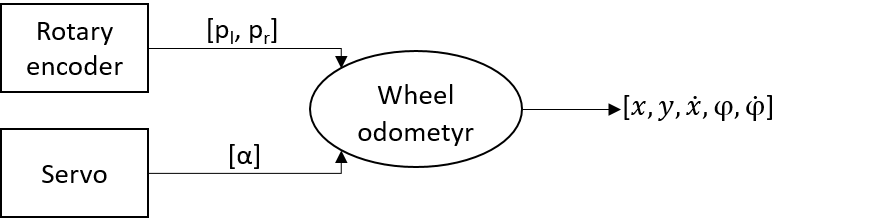
\includegraphics[scale=0.5]{odom_node}
        \label{fig:odom_pose}
    \end{subfigure}
    \begin{subfigure}{.5\textwidth}
        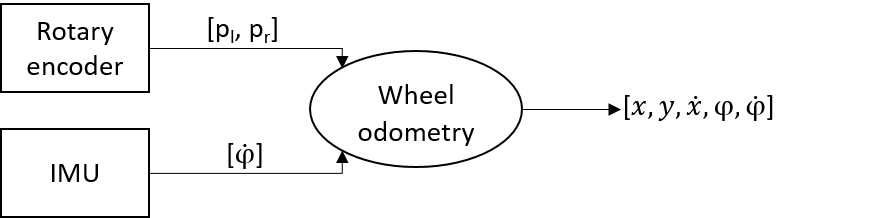
\includegraphics[scale=0.5]{odom_node_imu}
        \label{fig:odom_pose_imu}
    \end{subfigure}
    \caption{Wheel Odometry Node}
    \label{fig:odometry}
\end{figure}
\noindent Please note that, we assume there is no movement w.r.t roll, pitch angle and Z direction. Addition to this, there is not any velocity component in direction of y is "0" since the vehicle unable to catch any lateral force. Additionally, we calculating odometry in two different ways as shown in Figure \ref{fig:odometry}. First, we calculate the heading angle and rate using steering angle. Second, we use the IMU to get directly these two values without performing any mathematical effort. The result of these two approaches is presented in following section.

\section{Extended Kalman Filter}
In this section, the task is fusing IMU and odometry data. As mention in the previous chapter, we immigrate the EKF from ROS library into this thesis. Therefore, we have to only decide that which state we would like to estimate and what are our observation data from sensors. To proceed with EKF, we first introduce what state we can estimate and how we configure them in state estimation node \cite{kalman7}. In this node, the vehicle can be track in 15 different dimension like position, velocity and acceleration in 3D Cartesian coordinate system and in Euler angles as well as their rates as follows:
\begin{equation}\label{eq:state}
 \begin{bmatrix}
X & Y &Z\\
roll& pitch& yaw&\\
\dot X & \dot Y& \dot Z\\
\dot {roll} & \dot {pitch}& \dot {yaw}\\
\ddot X & \ddot Y& \ddot Z
\end{bmatrix}   
\end{equation}
\par In configuration phase, we should decide which parameter should be fused. As shown in figure \ref{fig:odometry}, the odometry node provides x, y position in the local reference frame, velocity and heading rate in the body frame, while IMU provides heading rates and linear acceleration in body frame w.r.t roll, pitch, yaw and x, y, z respectively.
\\
\begin{figure}[H]
    \centering
    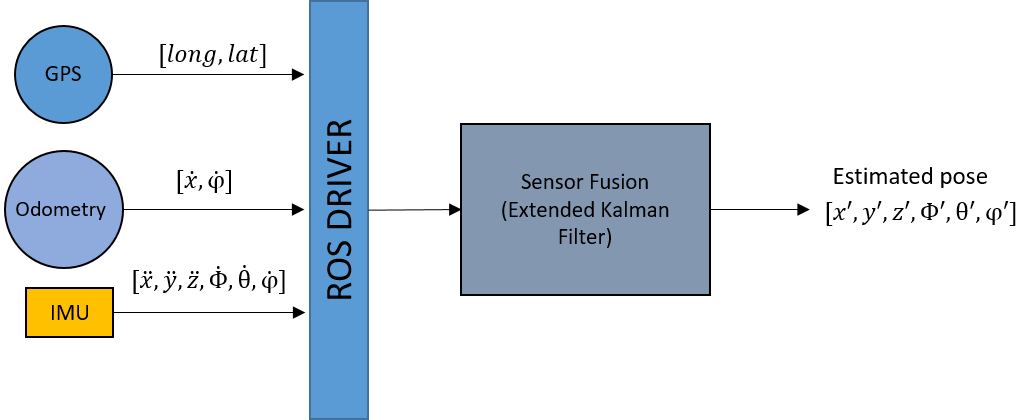
\includegraphics[width=\textwidth,height=6cm]{ekf.png}
    \caption{Caption}
    \label{fig:ekf_node}
\end{figure}
\newpage
We fuse the velocity and heading rate provided by odometry node along IMU data into state estimate node. It is important to note that, we do not fuse x, y parameter of odometry as long as IMU exist on the system. The reason is only avoiding to duplicate information since the velocity and absolute position of the vehicle calculated from the same source that may cause the filter to diverge from the desired value. You may also wonder why do we fuse the y component of the velocity ($\dot Y$), in spite of being mentioned as "0" at beginning of this chapter. At first glance, it does not make sense but it actually helps the filter to infer that there is no movement in the y-direction. At the end we have configuration matrix for every single sensor as follows:
\\
\begin{equation}\label{eq:config}
    \begin{bmatrix}
    false,&false,&false\\
    false,&false,&false\\
    true,&true,&false\\
    false,&false,&true\\
    false,&false,&false
    \end{bmatrix}
\end{equation}\\

\noindent where \textbf{\textit{false}} means the value will not be fuse while \textbf{\textit{true}} means the value will be fused. Note that the matrix in equation \eqref{eq:config} maps the matrix in equation \eqref{eq:state}

\par As a next and last step, we should tune the process and measurement noise co-variance matrices \textbf {Q} and \textbf{P},respectively. These two matrices are 15 by 15 size, diagonal and all its elements regard to state matrix. Here, the rule we should follow for setting \textbf {Q} and \textbf{P}: Assume that we would like tune EKF for one measuring parameter, so we have to change the value of the diagonal variable that corresponds to be fused parameter in Q and P matrix. Thus, we can influence the filter in a way that changes its fast to converge true value. For instance, if one can set the diagonal value of P matrix for velocity ($\dot X$) bigger than that measurement’s co-variance so, it makes the filter converge faster. On the other hand, if one can increase the diagonal value of Q matrix and hence it causes the error to grow faster in the state estimate part. Therefore, it effect filter converge faster in principle. However, it is very hard to tune both Q and P matrices but one can reach very optimal result by tuning them. In chapter \ref{sec:result}, it shows the affect of P and Q on EKF.

\section{Normal Distribution Transform}
This section, we describe how NDT method is applied in order to estimate pose in 6 degrees of freedom (DOF). This application is improved by pulling it from point clouds (PCL) and Autoware which are both open source libraries. The basic NDT algorithm is designed to use only point clouds information for finding  most likelihood transformation between the reference and target model as shown in figure \ref{fig:ndt}.
\begin{figure}[H]
    \centering
    \setlength{\fboxsep}{0pt}%
    \setlength{\fboxrule}{1pt}%
    \fbox{
    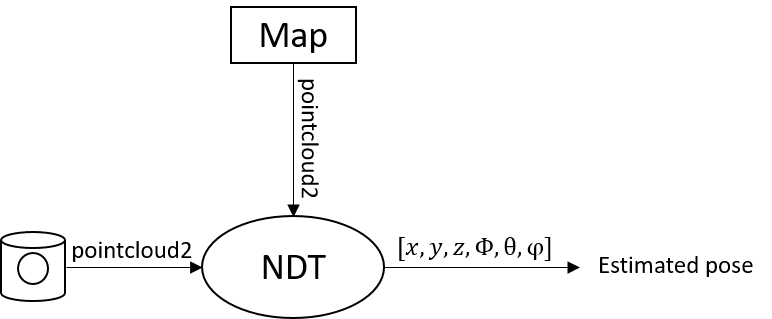
\includegraphics[scale=0.6]{ndt}}
    \caption{Workt Flow of the basic NDT algorithm} 
    \label{fig:ndt}
\end{figure}
NDT tries to extract the position of vehicle on the prior map. However, the basic NDT has a tendency to lose track of position against any disturbance for example, change of environment conditions. Therefore, we first link the odometry reading with NDT in order to support for tracking pose. We here note that we are not using position of odometry since it is not only prone to drift but also it uses different frame than NDT. Due to the fact, only the linear and angular velocity of odometry is used to recalculate the relative position. After that, the found position is added to the current position for correcting the estimated position of NDT. Subsequently, NDT node is redesigned as shown in figure \ref{fig:ndt_odom}.
\begin{figure}[H]
    \centering
    \setlength{\fboxsep}{0pt}%
    \setlength{\fboxrule}{1pt}%
    \fbox{
    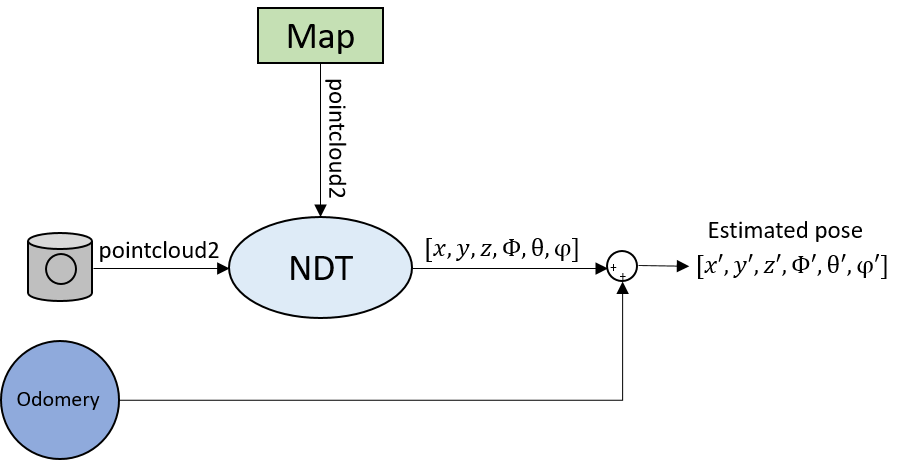
\includegraphics[scale=0.6]{ndt_odom}}
    \caption{Caption}
    \label{fig:ndt_odom}
\end{figure}
\par However, a further improvement of NDT is needed since odomerty has lack of information about the movement of vehicle and it is unreliable for long-term localization as we discussed in section \ref{sec:odom}. At this point, EKF is brought into play to support the algorithm in order to make it more robust. We employ EKF with odometry and IMU data to add NDT as shown in figure \ref{fig:ndt_ekf}.
\begin{figure}
    \centering
    \setlength{\fboxsep}{0pt}%
    \setlength{\fboxrule}{1pt}%
    \fbox{
    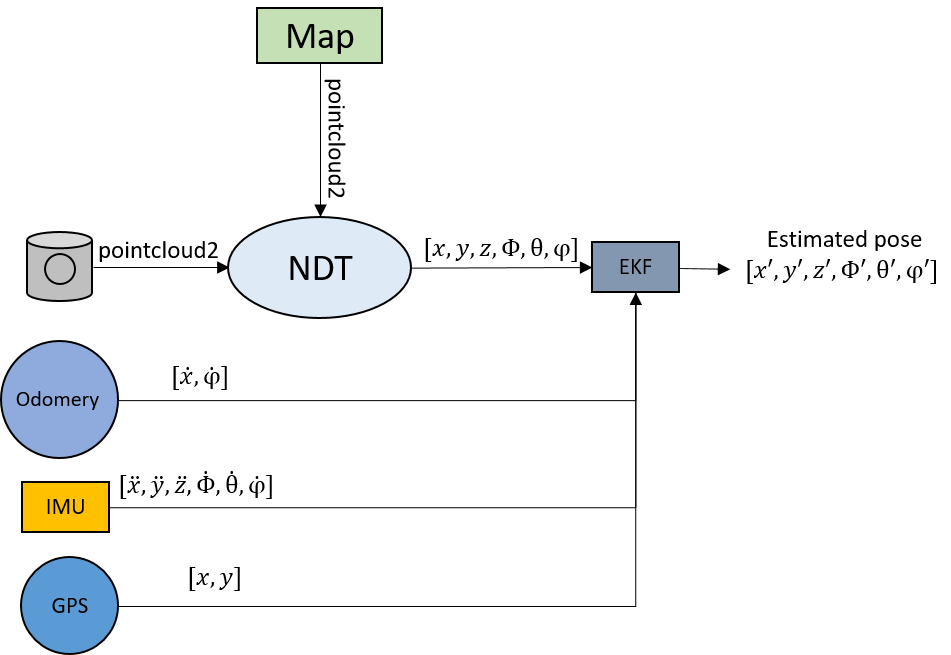
\includegraphics[scale=0.52]{ndt_ekf}}
    \caption{Caption}
    \label{fig:ndt_ekf}
\end{figure}
The advantage of employing EKF in this fashion is improving the result and removing the noise from sensors.
\par Yet there is another derivation of this application- In this instance, we use two EKF. One is used in the same way as the previous one. The other one is used for fusing NDT, IMU, and odometry as shown in figure \ref{fig:ndt_2ekf}. The purpose of doing this is eliminating unwanted movement of NDT since it estimates the pose of the vehicle in map frame hence it generates discrete jumps in a time period even though it eliminates drift \cite{rep105}. 
\begin{figure}[H]
    \centering
    \setlength{\fboxsep}{0pt}%
    \setlength{\fboxrule}{1pt}%
    \fbox{
    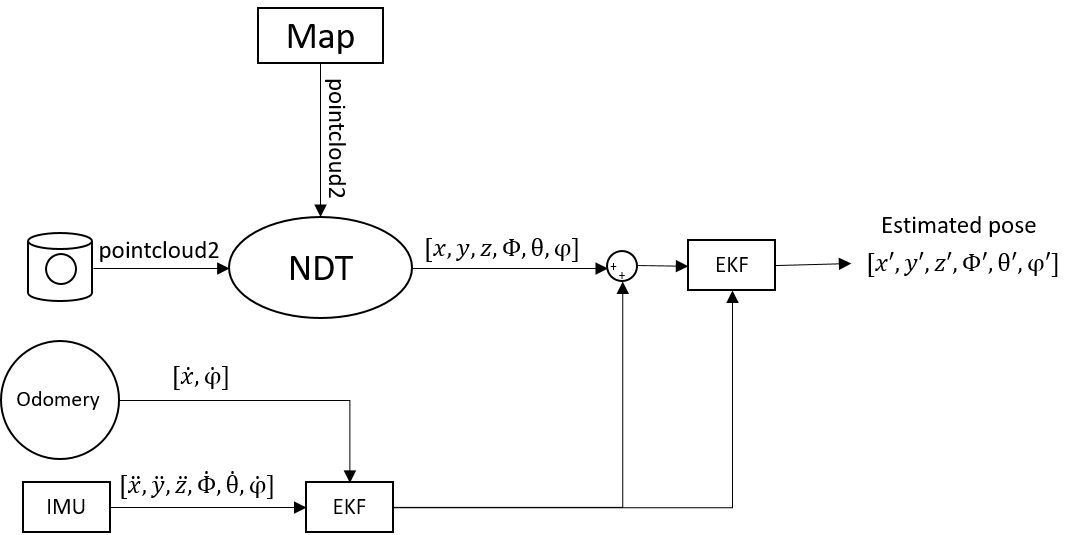
\includegraphics[scale=0.52]{ndt_2ekf}}
    \caption{Caption}
    \label{fig:ndt_2ekf}
\end{figure}

\par On the other hand, the algorithm is still not capable of self initialization. As mentioned in section \ref{sec:summary} is that NDT and ICP cannot find the matches between two scans unless they do know where to start. Therefore, we should provide a initial transform between the vehicle and the map. Thus, we approach this problem from GPS perspective. First, we provide static transformation between map and local coordinate by converting the first GPS output longitude and latitude, where a map is started to build, to Universal Transverse Mercator (UTM) coordinate by using geodetic tool \cite{utm}. Now, we have two transformations which are from GPS to map $_{M}^{G}T$ and GPS to vehicle $_{V}^{G}T$. Next step is finding transformation between map and vehicle $_{M}^{V}T$ by using chain rule property as follows \cite{robotic}:
\begin{align}
    _{M}^{G}T &= _{V}^{G}T \cdot _{M}^{V}T\\
    _{M}^{V}T &= _{V}^{G}T \cdot _{M}^{G}T^{-1}
\end{align}
It should be noted that the heading angle of the vehicle is provided from IMU for finding transformation  $_{M}^{V}T$ since GPS provides only longitude and latitude information.
\\
\par As a result of these improvements, NDT is transformed into a more robust algorithm than basic NDT as shown in figure \ref{fig:ndt_son}. Hence, NDT becomes more versatile to answer "where am I" and "where am I going" fundamental questions of robot navigation.  
\begin{figure}[H]
    \centering
    \setlength{\fboxsep}{0pt}%
    \setlength{\fboxrule}{1pt}%
    \fbox{
    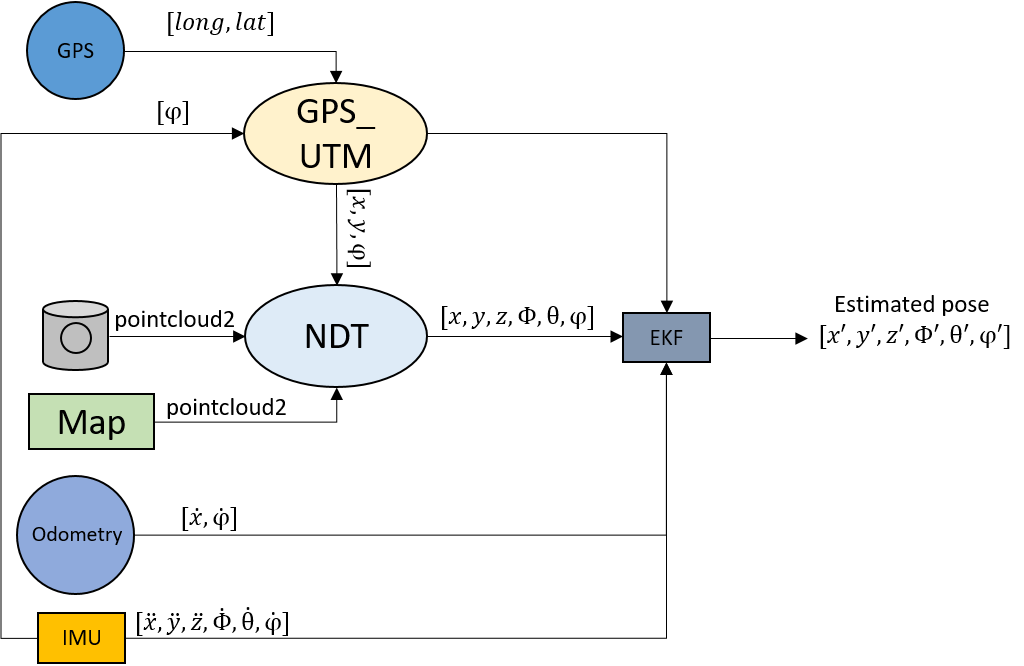
\includegraphics[scale=0.5]{ndt_son}}
    \caption{Caption}
    \label{fig:ndt_son}
\end{figure}
\section{Iterative Closest Points}
%----------------------------------------------------------------%
%-------------------------------CHAPTER5-------------------------%
\chapter{Experiments}\label{chp:5}
Finally, previously discussed methods in chapter \textbf{\ref{chp:3}}, \textbf{\ref{chp:4}} were tested and presented their results in the following sections by using different data sets. The purpose of this chapter is to evaluate those algorithms in terms of accuracy and robustness under real-world condition. Therefore, we conducted several experiments by using MIAcar. MIAcar is equipped pc and several sensors but we used only pc and three sensors in scope of this thesis as follows:
\begin{itemize}
    \item LIDAR\footnote{\url{https://velodynelidar.com/hdl-32e.html}}
    \item IMU-GPS \footnote{\url{https://www.xsens.com/products/mti-g-710/}}
    \item Magnetic encoder
    \item PC (i7 processor with 16GB RAM)
\end{itemize}
and their setups are shown in figure \ref{fig:setup}.
\\
\begin{figure}[ht]
    \centering
    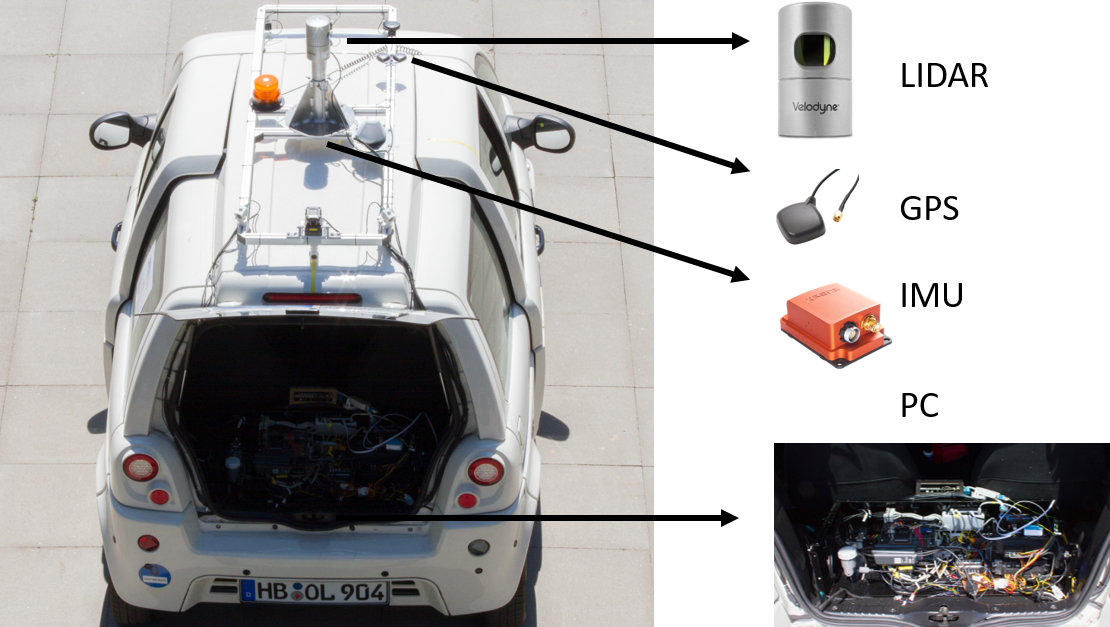
\includegraphics[scale=0.6]{mia2}
    \caption{Sensor setup configuration on MIAcar}
    \label{fig:setup}
\end{figure}


\newpage
Alternatively, we also tested these algorithms with another dataset which is called KITTI (Karlsruhe Institute of Technology and Toyota Technological Institute). This data set is promoted as a benchmark to validate any localization algorithms \cite{kitti}.
\par To continue, we organized this chapter as follows: In Section \textbf{\ref{sec:Exp}}, we explained the experimnetal setups and show the preliminary works. We then presented the results  of MIA and KITTI in Section \textbf{\ref{sec:MIA-set}} and \textbf{\ref{sec:KITTI-set}}, respectively.

\section{Experimental Procedure}\label{sec:Exp}
To cover different aspects of real-world conditions, experiments should be designed in a wide spectrum. Therefore, we conducted several experiments in different environments and different weather conditions as much as possible. However, we must do some preparations which are always need to be considered in order to conduct a proper experiment. For this reason, we described the required works in the following section. 

\subsection{Preliminary Work}
\subsection*{Sensor Positioning} 
The first task was to determine the position of sensors w.r.t center of the vehicle, in particular, LIDAR and IMU. Since the main localization algorithm that used in this thesis affiliates with LIDAR and IMU, thereby the position of these sensors had a big impact on results. Thus, the preliminary works on these sensors setup highly important in order to have concrete results from localization algorithms and having an accurate 3D map.
\subsection*{Map Construction}\label{mapping}
Once the positions of sensors were determined and set them up correctly, the second work was to build a map of the environment where the experiment would be carried out. For this purpose, the car was first driven in a test area to collect the related sensory data e.g. point clouds for creating a three-dimensional map as shown in figure \ref{fig:rh_3d}.
\par To create 3D map, we used NDT algorithm in the same manner as mentioned in \cite{ndt_map}. The working principle of NDT is almost the same as the localization algorithm, except it saves every scan match in space instead. Of note, this method is very time intensive for building map even though it provides a relatively accurate map. Nevertheless, the created map was used for the course of this thesis.

\begin{figure}[t!]
\subfloat[3D Map of Robert-Hooke-Straße in Bremen \label{fig:rh_3d}] {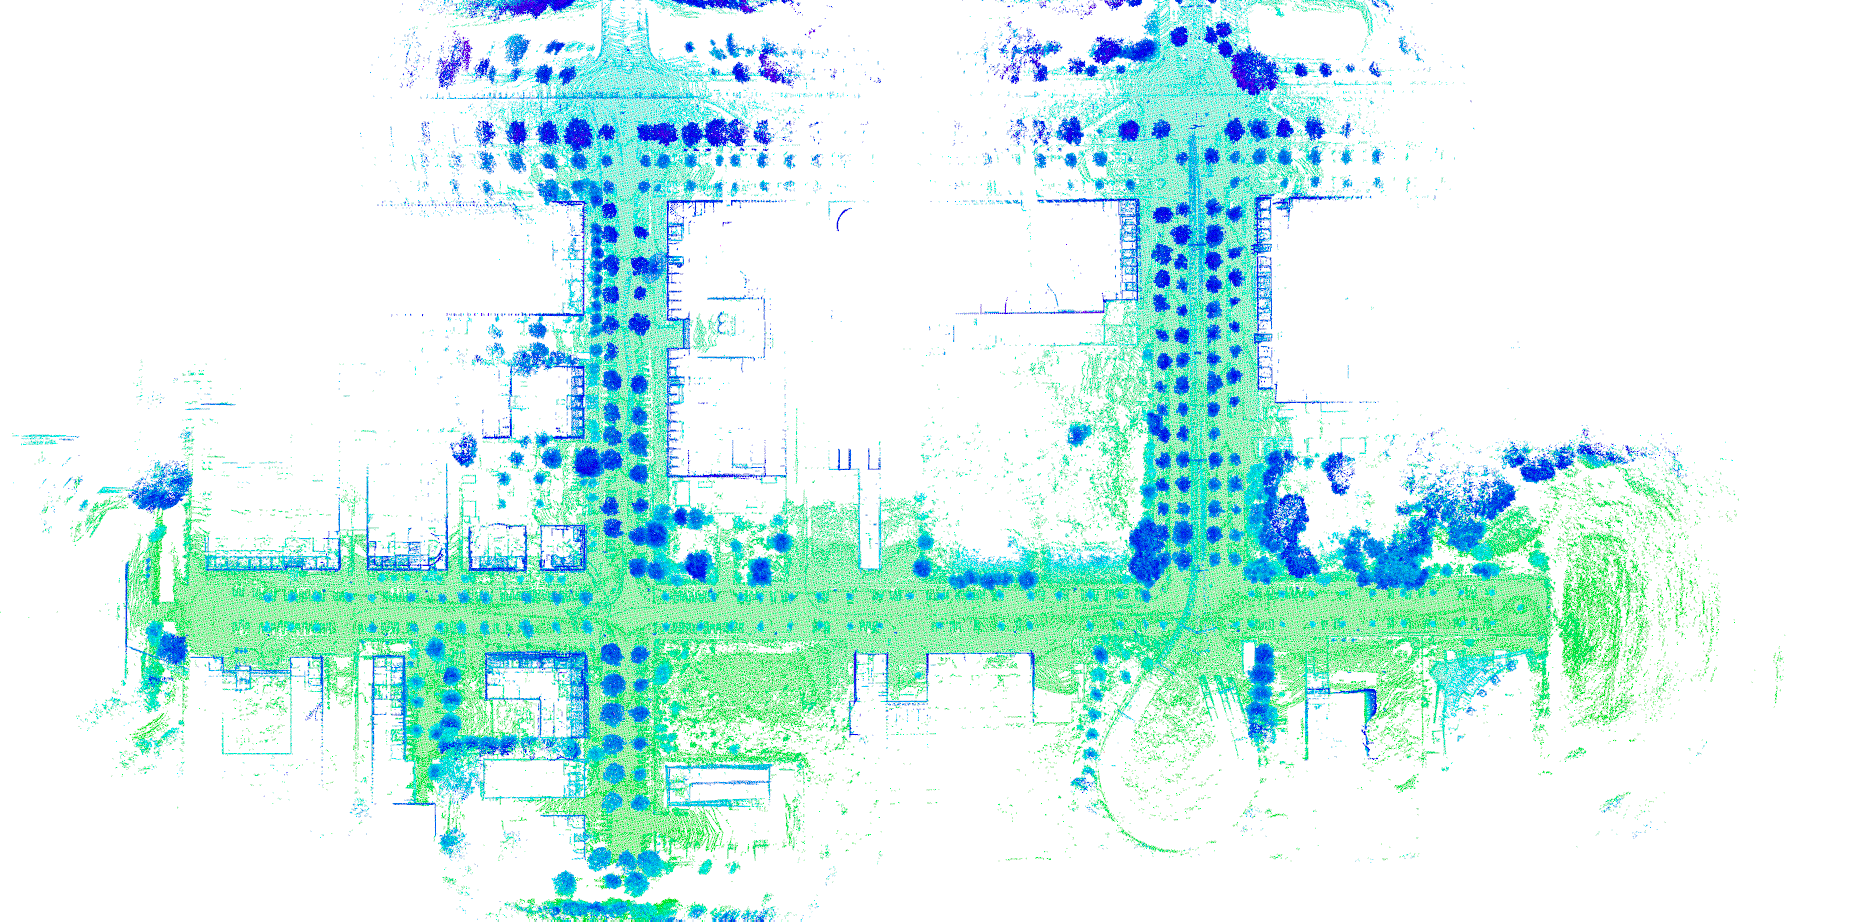
\includegraphics[width=\textwidth]{rh_3d}}\\
\subfloat[The bird view of Robert-Hooke-Straße in Bremen \label{fig:rh_google}]{\includegraphics[width=\textwidth]{rh5_google}}
\label{fig:comparison}
\caption{Comparing the created 3D map (a) and real map (b)}
\end{figure}

\newpage
\subsection*{Down Sampling}
The final task was concerning to decrease the computational time of the map-based localization algorithm. As it was previously discussed, the most preferable way to keep the execution time in optimum level is to down-sample both data that obtained from map and LIDAR. By this way, we also decreases the complexity of the map and distribute LIDAR points evenly (see figure \ref{fig:vox_size}) \cite{ndt_map}. In figure \ref{fig:no_filter}, the map contains a large amount of redundant information i.e. the surface of objects in the map are represented by a set of points that are more than needed to depict the surface of the object. Therefore, the original map was needed to be down-sampled as shown in figure \ref{fig:filter_rh}.

\begin{center}
\begin{figure}
\subfloat[\textbf{Original Map:} 3D map of the area was generated (offline) from recorded LIDAR sensor data. It contains 71,120,230 points of 1GB size.
\label{fig:no_filter}] {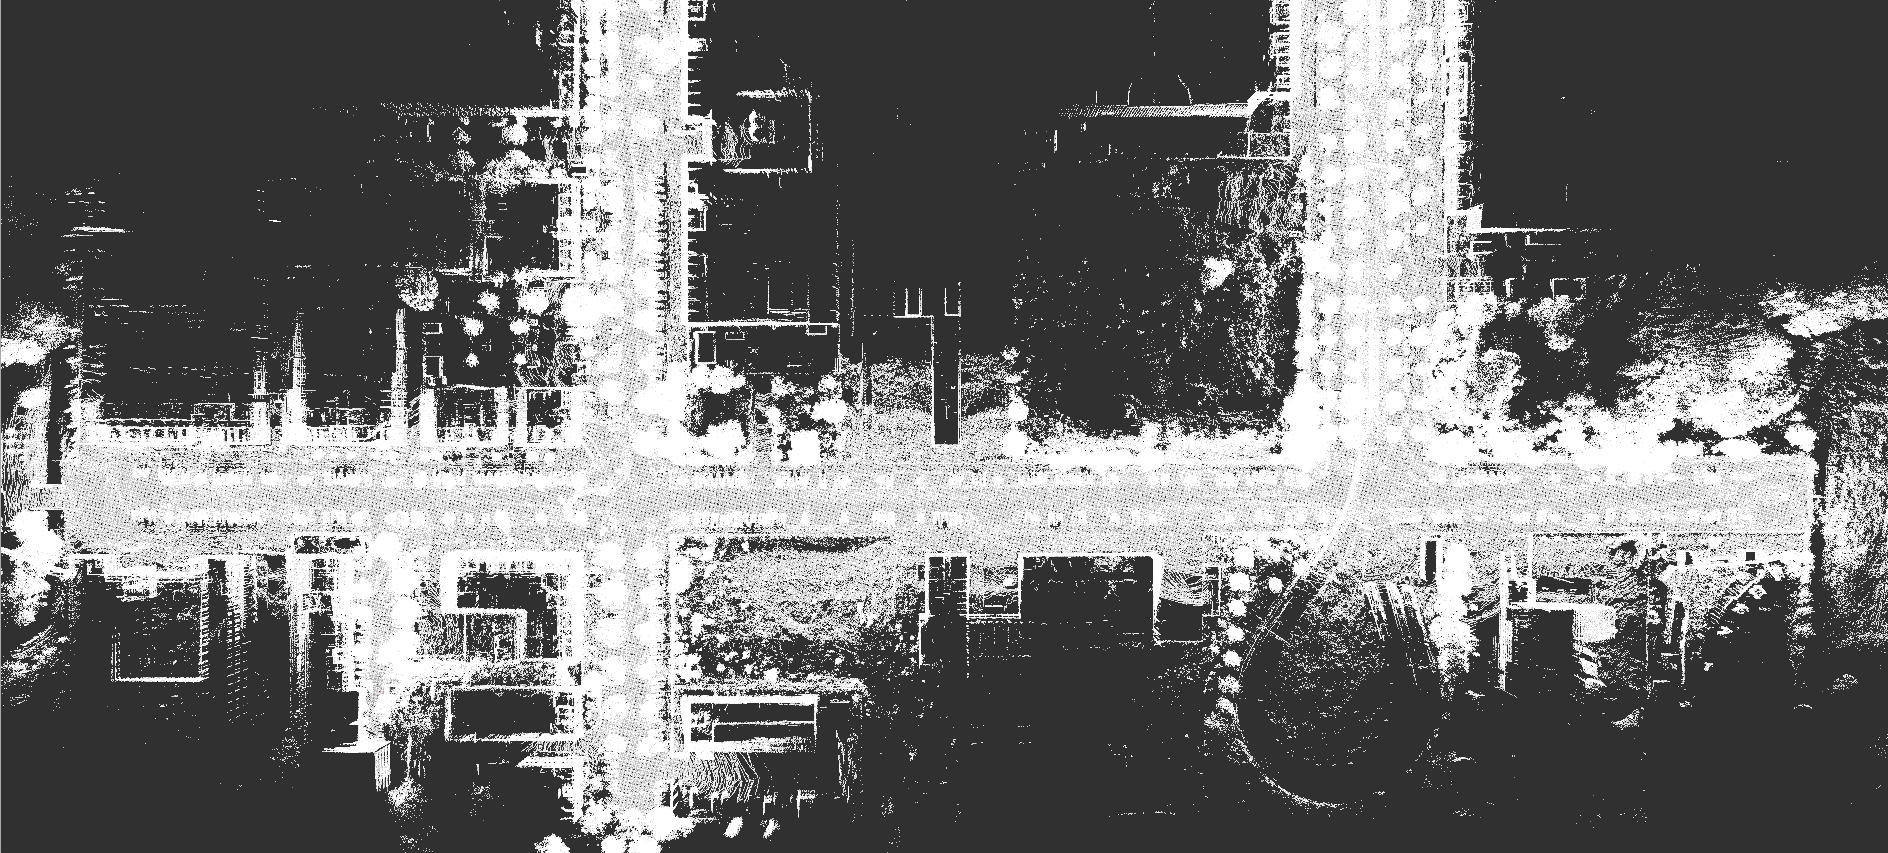
\includegraphics[scale=0.3]{no_filter}}\\
\subfloat[\textbf{Down-sampled Map:} After down-sampled process (filter size 0,5m), map contains 1,110,350 points of 17,8MB size \label{fig:filter_rh}]{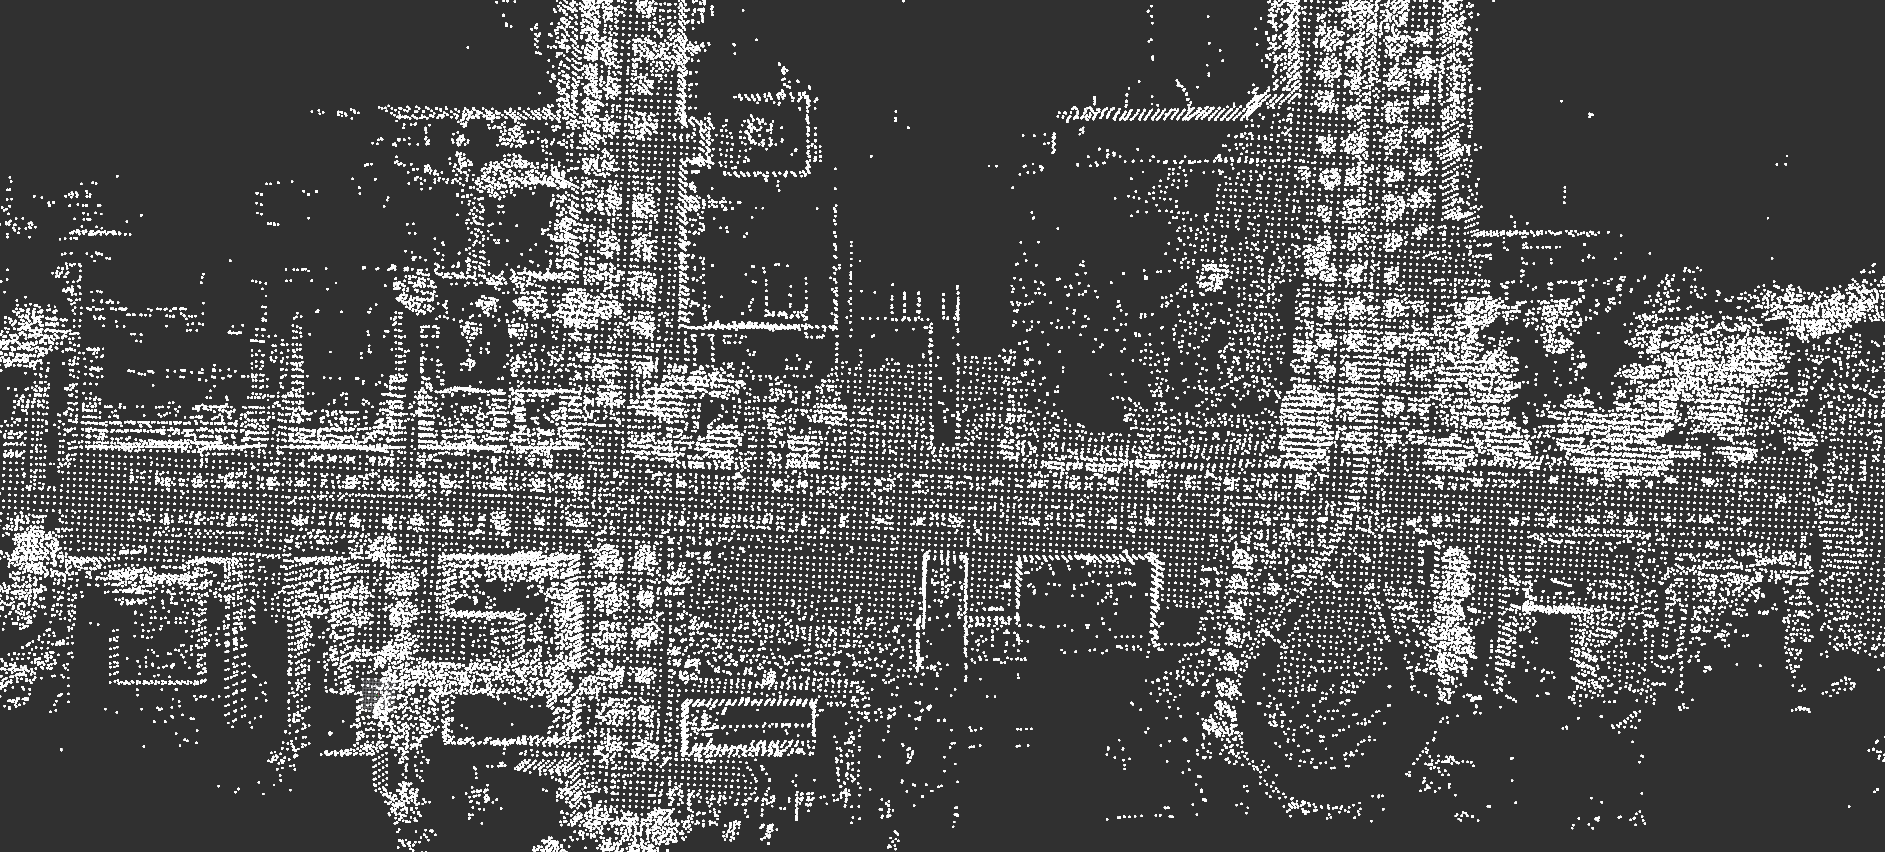
\includegraphics[scale=0.3]{filtered_rh}}
\label{fig:filter}
\caption{Illustration of orginal map (a) and down-sampled map (b) }
\end{figure}
\end{center}

\begin{figure}[t]
\subfloat[Voxel size = 0 m]{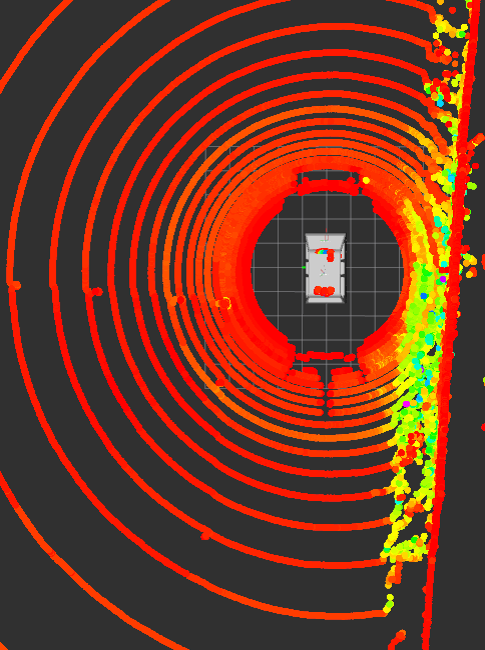
\includegraphics[scale=0.5]{0}}\hfill
\subfloat[Voxel size = 1 m]{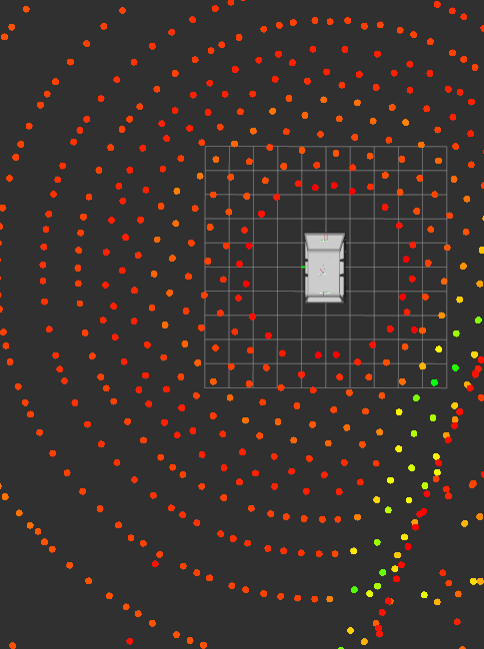
\includegraphics[scale=0.5]{1}}\hfill
\subfloat[Voxel size = 2 m]{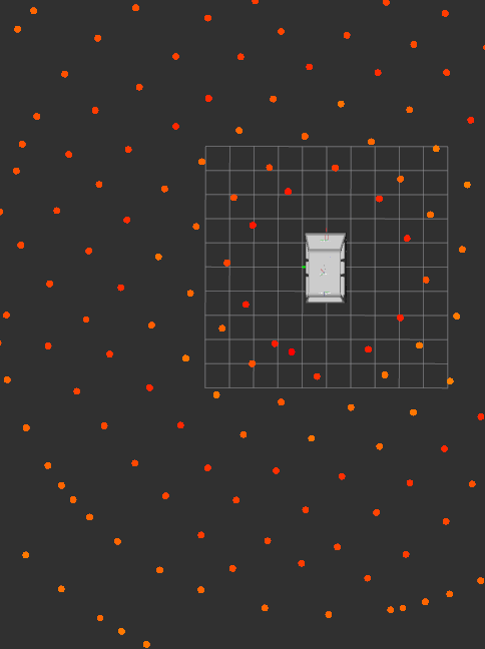
\includegraphics[scale=0.5]{2}}\\
\subfloat[Voxel size = 3 m]{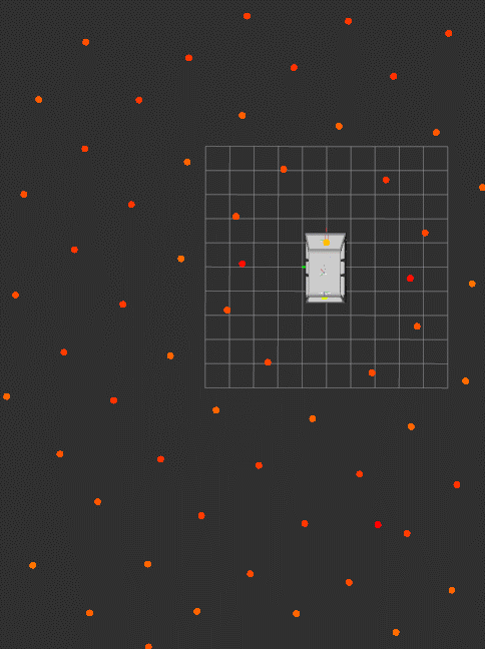
\includegraphics[scale=0.5]{3}}\hfill
\subfloat[Voxel size = 4 m]{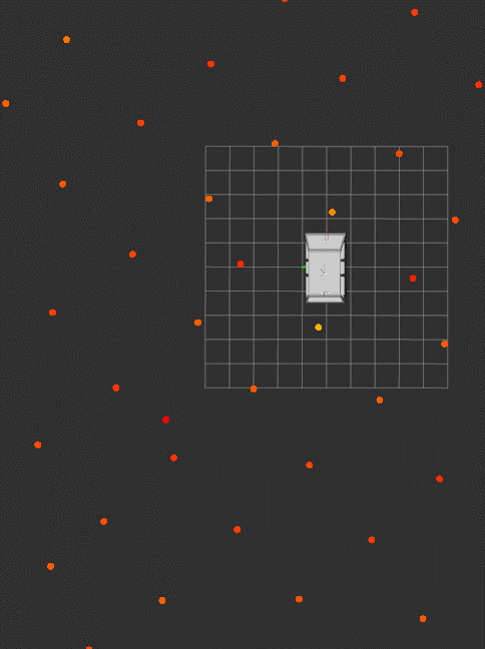
\includegraphics[scale=0.5]{4}}\hfill
\subfloat[Voxel size = 5 m]{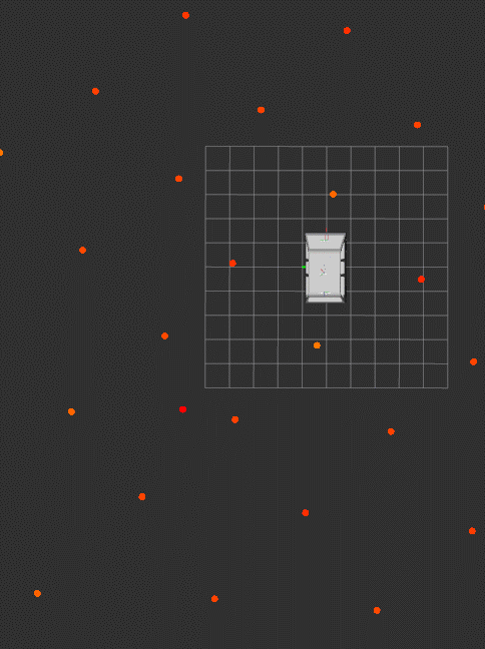
\includegraphics[scale=0.5]{5}}\hfill
\caption{Distribution of laser points over the different size of voxel}
\label{fig:vox_size}
\end{figure}
\vspace{-1cm}
\par To down-sample, we used an algorithm that was provided by \acrfull{ros} is Voxel-filter\footnote{\url{http://wiki.ros.org/pcl_ros}}%comment:The VoxelGrid class creates a 3D voxel grid (think about a voxel grid as a set of tiny 3D boxes in space) over the input point cloud data. Then, in each voxel (i.e., 3D box), all the points present will be approximated (i.e., downsampled) with their centroid. This approach is a bit slower than approximating them with the center of the voxel, but it represents the underlying surface more accurately.
. The concept of this filter is to find the centroid of points $(C_{x}, C_{y})$ within voxel cell as described in the following equations:\\
\begin{equation}
C_{x} =\dfrac{1}{6A}\sum_{i=0}^{n-1}(x_{i}+x_{i+1})(x_{i}y_{i+1}-x_{i+1}y_{i})
\end{equation}
\begin{equation}
C_{y} =\dfrac{1}{6A}\sum_{i=0}^{n-1}(y_{i}+y_{i+1})(x_{i}y_{i+1}-x_{i+1}y_{i})
\end{equation}\\
and where A is the polygon's signed area as described by \cite{centroid},
\begin{equation}
A =\dfrac{1}{2}\sum_{i=0}^{n-1}(x_{i}y_{i+1}-x_{i+1}y_{i})
\end{equation}

\section{MIA Dataset}\label{sec:MIA-set}
MIA dataset was  created by driving the car around Robert-Hooke-Straße, Jeddeloh driver training area and Bassum go-kart track. Dataset consist of LIDAR, IMU, wheel rotation, RGB image and radar information.
\subsection{Robert-Hooke-Straße Test} The first test was carried out in a place where the road condition was asphalt and the weather was sunny. The vehicle was driven around in this place approximately \textbf{2167} meter (m) (see figure \ref{fig:rh_gps}) and the result of algorithms was evaluated by collected raw data.
\\
\begin{figure}[ht]
    \centering
    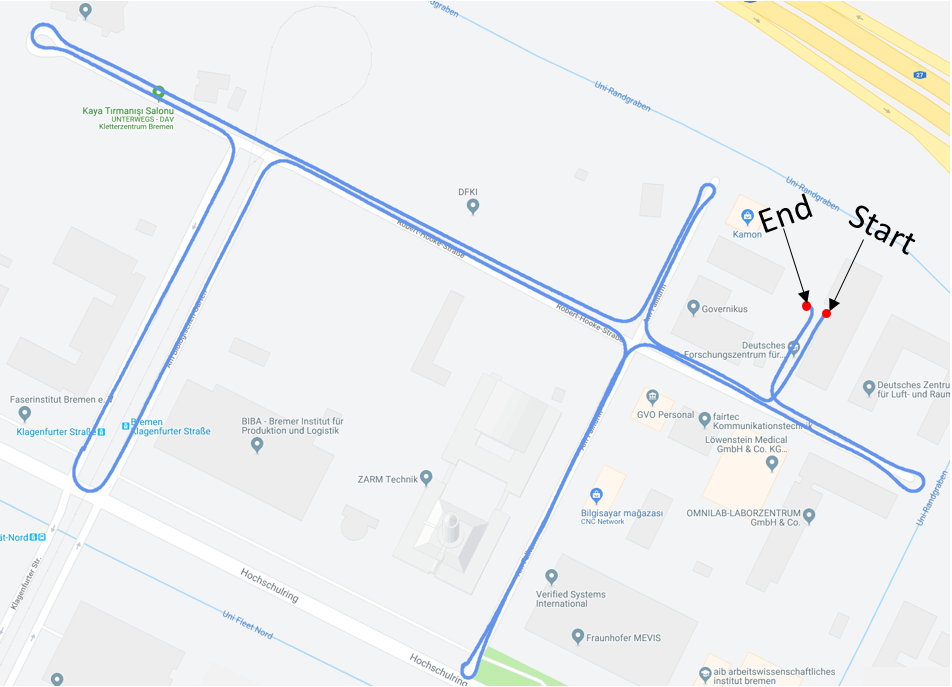
\includegraphics[scale=0.50]{rh_gps}
    \caption{The bird view of the first test area. The vehicle was driven manually for data acquisition on the blue line which indicates the GPS trace}
    \label{fig:rh_gps}
\end{figure}

\noindent \textbf{Assessment of the Idea:} All the obtained result including translations and rotations errors were evaluated by comparing them with ground truth which was obtained via NDT algorithm under the following conditions:
\begin{itemize}
    \item Map resolution 0.2 m,
    \item Source resolution 1 m.
\end{itemize}

As seen on the plots below, pure wheel odometry (a) and improved odometry (b) described in \ref{sec:wheel_odometry} were compared with the ground truth. It is quite clear that using heading velocity from IMU sensor enhances the quality of the wheel odometry about \textbf{30} \%. Nevertheless, error of wheel odometry was more larger than  upper limit for autonomous driving. On the graph \ref{fig:odom_compare_all}, we presented overall comparison between odometry and the ground truth.
\begin{figure}[H]
\centering
\subfloat[\small Performance of pure wheel odometry against ground truth in 3D showed as translation and rotation errors]{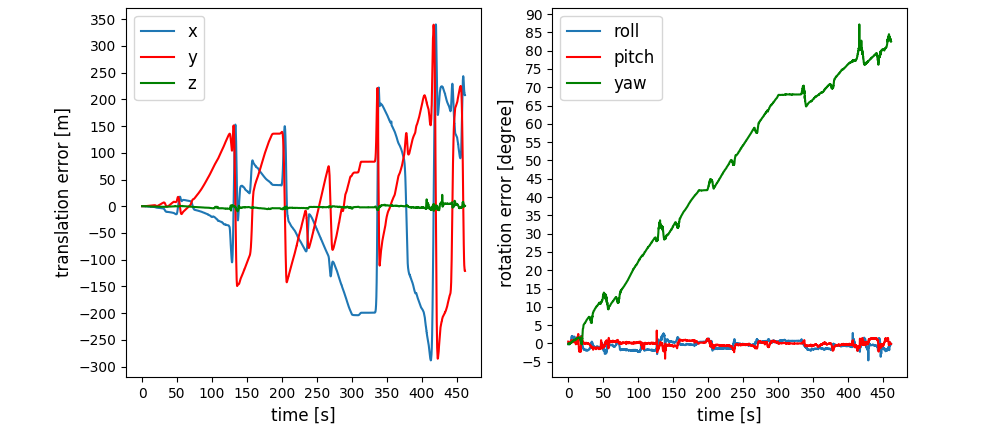
\includegraphics[height=5cm,width=\textwidth]{odom_error}}\\
\subfloat[\small Performance of wheel odometry with IMU against ground truth in 3D showed as translation and rotation errors]{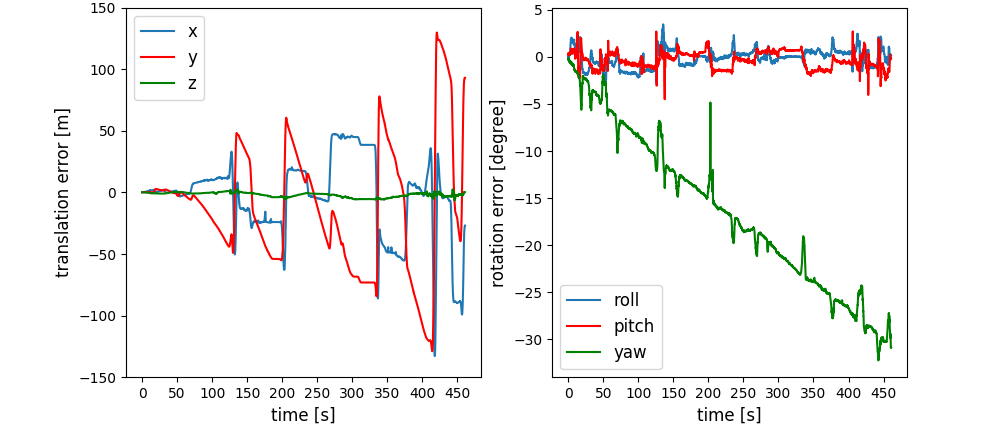
\includegraphics[height=5cm,width=\textwidth]{odom_imu_error}}
\label{fig:wheel_compare}
\end{figure}
\vspace{-0.5cm}
\begin{figure}[H]
    \centering
    \subfloat[\small {Overall comparison between ground truth (blue), steering-wheel-based wheel  odometry(red) and IMU-based wheel odometry (green)}]{\label{fig:odom_compare_all}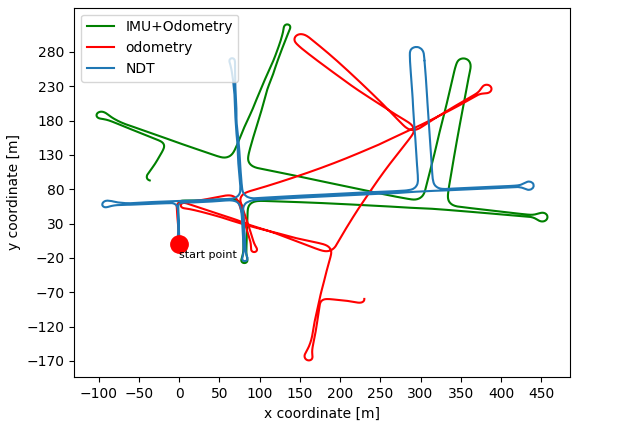
\includegraphics[scale=0.4]{ndt_imu_odom_compare.png}}
    \caption{Comparison between odometry and ground truth}
    \label{fig:my_label}
\end{figure}

\par Next task was improving wheel odometry by fusing IMU and GPS data. For this purpose, the performance of EKF was tested by integrating linear and heading velocity ($V_x, V_y, \dot{\theta}$), x-y positions, angular velocities ($\dot {roll}, \dot {pitch}, \dot {yaw}$) and acceleration ($\ddot X, \ddot Y, \ddot Z$) from wheel odometry, GPS and IMU, respectively. 
\begin{figure}[H]
    \centering
    \subfloat[General view of comparison between EKF (red) and ground truth (blue)]{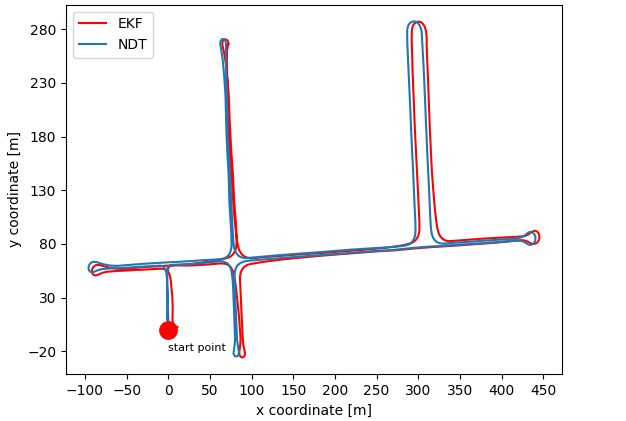
\includegraphics[scale=0.4]{ekf_vs_ndt}\label{fig:ekf_vs_ndt}}
\end{figure}
\vspace{-0.5cm}
\begin{figure}[H]
    \centering
    \subfloat[\small{Performance comparison between EKF together with GPS, IMU, Odometry and ground truth in 3D showed as translation and rotation errors }]{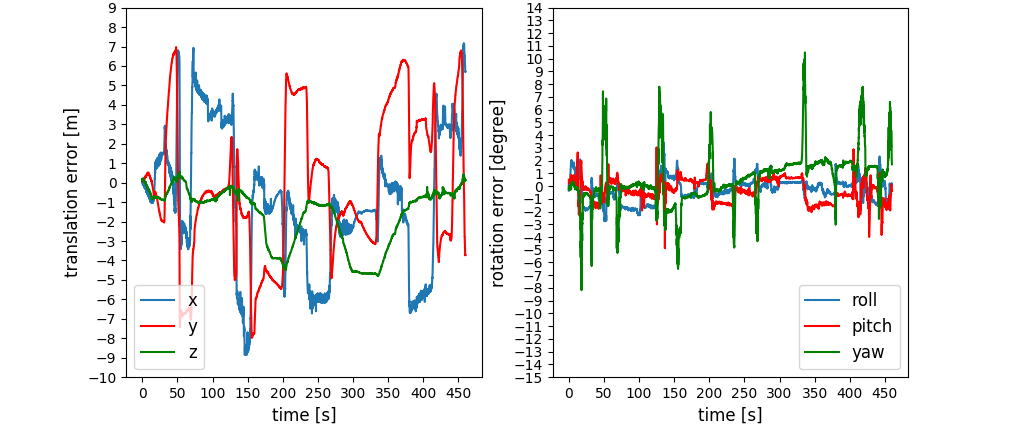
\includegraphics[height=5cm,width=\textwidth]{ekf_error}\label{fig:ekf_error}}
    \caption{Comparison between EKF and ground truth}
    \label{fig:ekf_graph}
\end{figure}
\noindent Despite good performance (see figure \ref{fig:ekf_graph}) of EKF compared with previous example, the overall performance of EKF was not as precise as the ground truth as shown figure \ref{fig:ekf_vs_ndt}.

\par Before proceeding the final test, we had to make a decision between two scan registration methods to have more efficient and robust localization. Therefore, we conducted another test to evaluate their performance against each other in terms of execution time, translation, and rotation differences.\\ 
\par Of note, to make a fair test, we should use the same map whose voxel size 2 m. However, we found out that NDT algorithm cannot handle sparse map, while ICP worked much more successfully. In contrast, ICP could not make any progress on a relatively intensive map, while NDT worked seamlessly. Thus, we had to use two different maps but we set the common parameters of two methods exactly the same to keep the test as fair as possible.
\begin{itemize}
\item Common parameters
\begin{itemize}
    \item down-sampled source scan (LIDAR) by 2m voxel size,
    \item same initial translation and rotation error (both initialized by GPS),
    \item same number of iterations 50.
\end{itemize}
\end{itemize}

\begin{figure}[H]
\centering
\subfloat[General view of comparison between ICP (red) and NDT (blue), in side of the boxes the overlap showed at higher magnification]{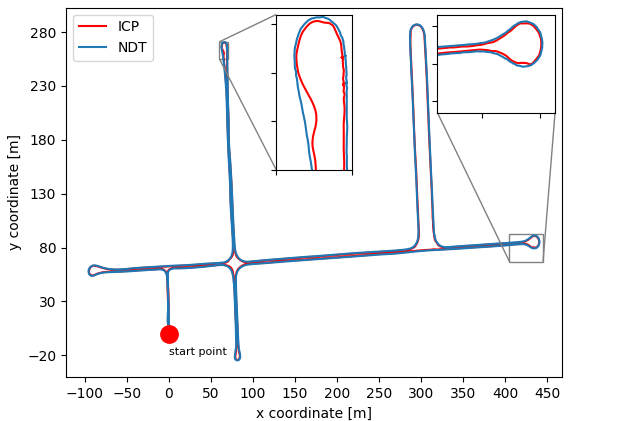
\includegraphics[scale=0.4]{icp_vs_ndt}\label{icp_mag}}
\end{figure}
\vspace{-0.5cm}
\begin{figure}[H]
\centering
\subfloat[Performance comparison between NDT and ICP in 3D showed as translation and rotation error ]{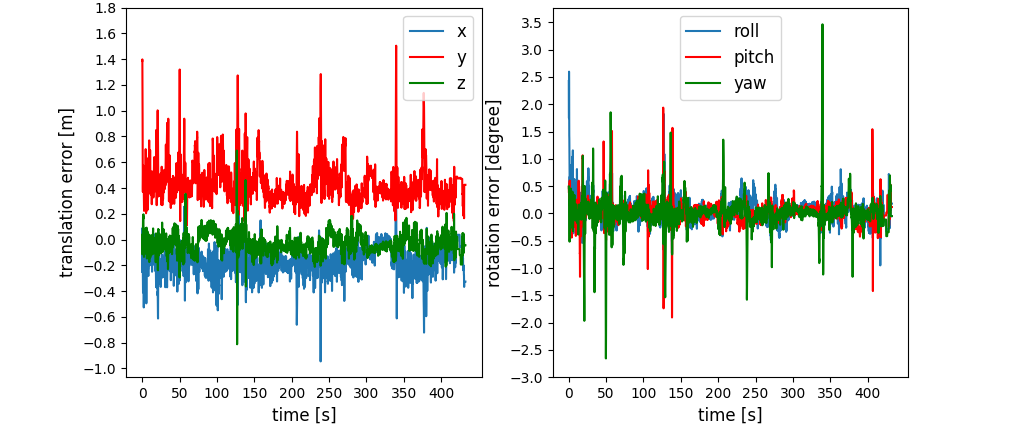
\includegraphics[height=5cm,width=\textwidth]{error_icp}}
\caption{Comparison between two scan registration algorithm NDT and ICP}
\label{fig:icp_vs_ndt}
\end{figure}
\begin{table}[H]
    \centering
    \small
    \begin{tabular}{|c|c|c|c|}
    \hline
         methods &resolution of map [m]&filter size of source [m]&exec. time [s]\\ 
         \hline
         ICP& 2& 2 & 89.80\\
         \hline
         NDT& 0.2 & 2 & 31.63\\
         \hline
    \end{tabular}
    \caption{Execution time of methods under the certain condition}
    \label{tab:compare_ekf_ndt}
\end{table}

It is fairly clear that ICP has a tendency to go inside to keep the overlap area as much as it can ( seen figure \ref{icp_mag}). It also can be clearly seen that ICP could not find the proper transformation as good as NDT between target and source scan when the vehicle made u-turn. Another aspect of this comparison is observing the execution time of both methods which was stated in table \ref{tab:compare_ekf_ndt} under the certain conditions such as map resolution and filter size. The execution time is playing a distinct role in deciding to which method used primarily for supplying proper localization less 100 ms since it is the sampling time of the LIDAR sensor.

\newpage
\par Finally, we tested the method as shown in figure \ref{fig:ndt_son}, which combines the EKF with NDT, under the following condition:
\begin{itemize}
    \item Map resolution 0.75 m,
    \item Source resolution 3 m,
    \item initial state of EKF 0.5 m $x$, 0.05 m $y$ and -0.03 rad $\theta$
\end{itemize}
By doing this, we aimed to make NDT methods less sensitive about the density of map and to eliminate any possible fluctuation on localization (see figure \ref{fig:ekf_ndt_vs_ndt}).

\begin{figure}[H]
\centering
\subfloat[General view of comparison between combination of EKF with NDT (red) and NDT (blue), in side of the boxes  the elimination of vibration showed at higher magnification]{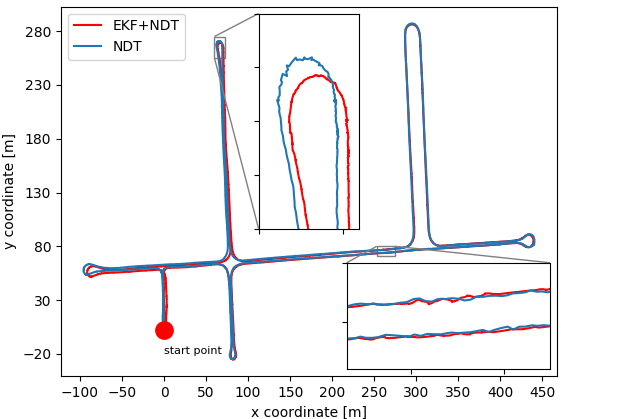
\includegraphics[scale=0.4]{ekf_ndt_vs_ndt}}
\end{figure}
\vspace{-0.5cm}
\begin{figure}[H]
\subfloat[Performance comparison between combination of EKF with NDT and NDT in 3D showed as translation and rotation errors]{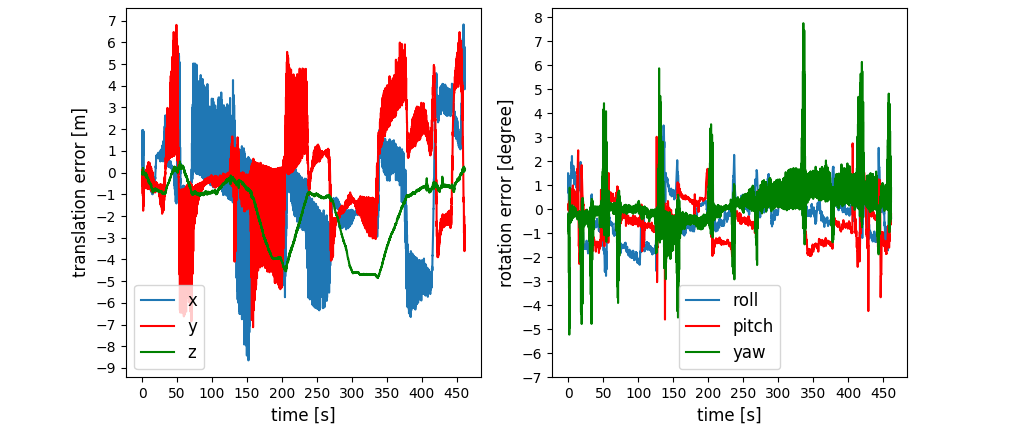
\includegraphics[height=5cm,width=\textwidth]{error_ekf_ndt_vs_ndt}\label{error_ekf_ndt}}
\caption{Comparison between combination of EKF with NDT and NDT}
\label{fig:ekf_ndt_vs_ndt}
\end{figure}

\begin{table}[H]
    \centering
    \small
    \begin{tabular}{|c|c|c|c|c|c|}
    \hline
         translation &max e.[m]&RMSE[m]&rotation&max e. [deg]&RMSE[deg]\\ 
         \hline
         x &8.65114&2.44113& roll  &3.48991&0.94101\\
         \hline
         y &7.12333&2.26043& pitch &4.59713&0.93819\\
         \hline
         z &4.85689&2.27955& yaw   &7.74988&0.99059\\
         \hline
    \end{tabular}
    \caption{Error calculation data which was subtracted from figure \ref{error_ekf_ndt}}
    \label{tab:compare_ekf_icp}
\end{table}
Additionally, we tested the combination of EKF with ICP as shown in the plots below.
\begin{figure}[H]
\centering
\subfloat[General view of comparison between combination of EKF with ICP (red) and ICP (blue), in side of the boxes  the elimination of vibration showed at higher magnification]{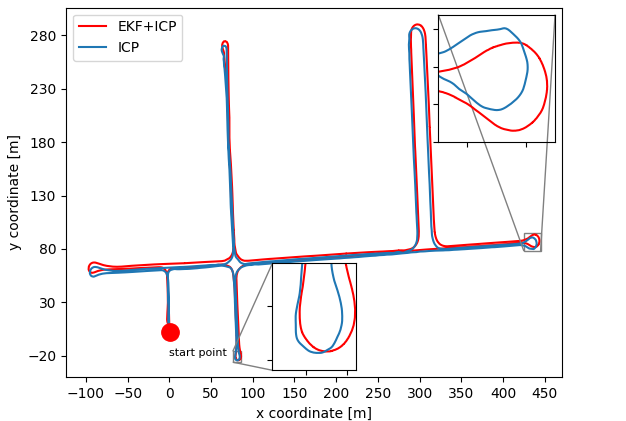
\includegraphics[scale=0.4]{ekf_icp_vs_icp}}
\end{figure}
\vspace{-0,5cm}
\begin{figure}[H]
\subfloat[Performance comparison between combination of EKF with ICP and NDT in 3D showed as translation and rotation error]{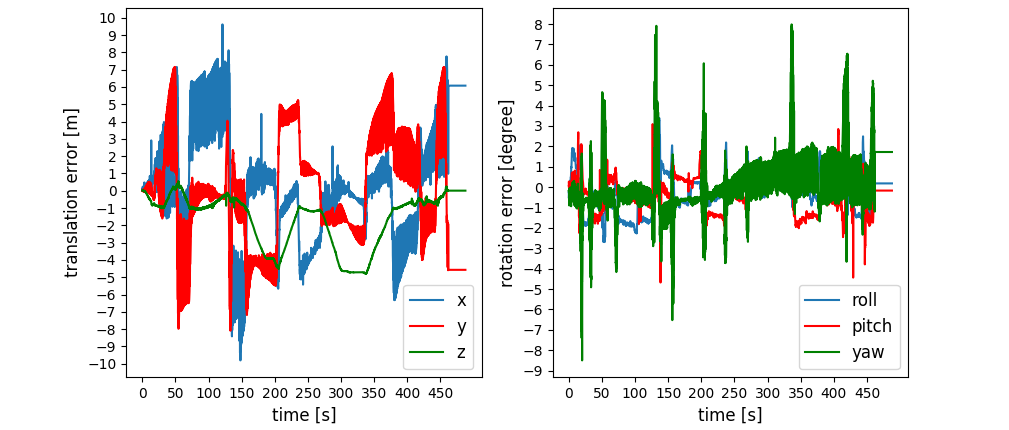
\includegraphics[height=5cm,width=\textwidth]{error_ekf_icp_vs_ndt}\label{error_ekf_icp}}
\caption{Comparison between combination of EKF with ICP and ICP}
\label{fig:ekf_icp_vs_icp}
\end{figure}

\begin{table}[H]
    \centering
    \small
    \begin{tabular}{|c|c|c|c|c|c|}
        \hline
         translation &max e.[m]&RMSE[m]&rotation&max e. [deg]&RMSE[deg]\\          \hline
         x &9.80437&3.60233& roll  &3.39731&0.92542\\
         \hline
         y &8.08773&3.42366& pitch &4.68054&0.91935\\
         \hline
         z &4.79653&2.21747& yaw   &8.50213&1.68752\\
         \hline
    \end{tabular}
    \caption{Error calculation data which was subtracted from figure \ref{error_ekf_icp}}
    \label{tab:exec_time}
\end{table}
\noindent EKF has done its task to eliminate all possible fluctuations on localization data. However, as it seen in figure \ref{fig:ekf_ndt_vs_ndt} and \ref{fig:ekf_icp_vs_icp}, there is a difference between EKF result and ground truth due to improper use of Kalman parameters. Table \ref{tab:compare_ekf_icp} and \ref{tab:exec_time} show the error calculation in term s of absolute maximum and mean translation and rotation error.
\subsection{Jeddeloh driver training area Test} The second test was carried out in a place where the road condition was gravel and weather was drizzle. The vehicle was driven in this place approximately 796 m (see figure \ref{fig:jeddeloh_gps}) and the obtained results of the algorithms was evaluated in the same manner as the previous example.
\\
\begin{figure}[H]
    \centering
    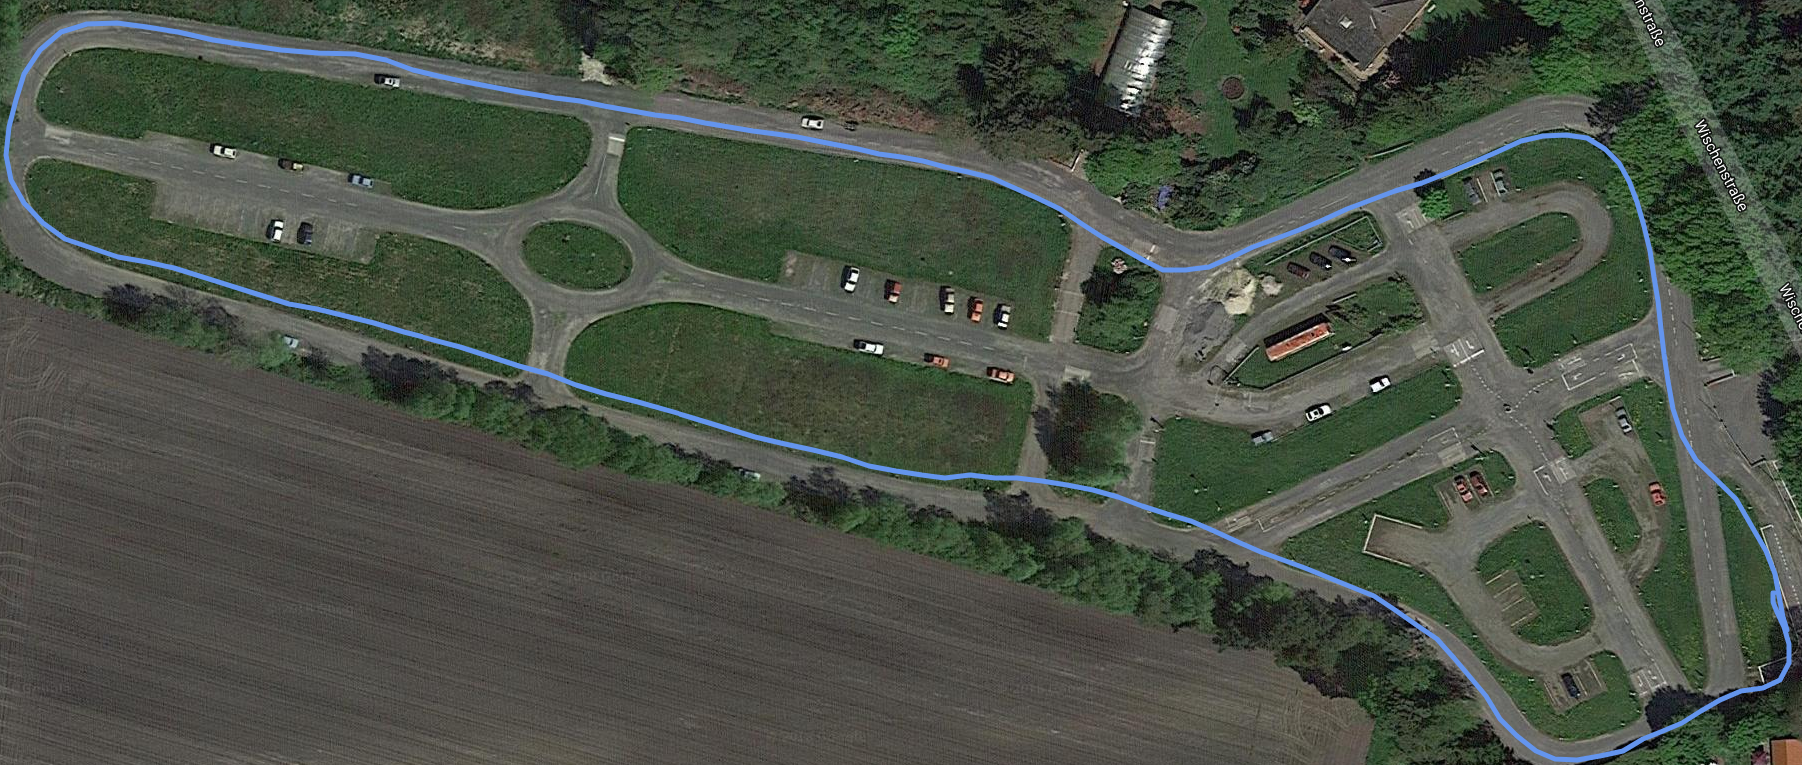
\includegraphics[scale=0.23]{jeddloc_gps}
    \caption{The bird view of the second test area. The vehicle was driven manually for data acquisition on the blue line which indicates the GPS trace}
    \label{fig:jeddeloh_gps}
\end{figure}
\noindent\textbf{Assessment of the Idea:} In this part, we only presented the final result which was provided by the combination EKF with NDT  as shown in figure \ref{fig:jeddeloh_error}. 
In this experiment, we realized that the process and measurement noise co-variance matrices of EKF was needed to be reconfigured due to the different road condition that was chosen for this experiment. Since the vehicle was driven on uneven terrain, in our case the it was gravel, it has a great impact on the measurement of the wheel odometry and IMU. In this sense, we chose Q smaller than the previous example in order to mitigate this effect. As a result of this, the combination of EKF with NDT algorithm delivered a relatively good result as stated in table \ref{tab:jeddeloh}. 
\\
\begin{figure}[H]
    \centering
    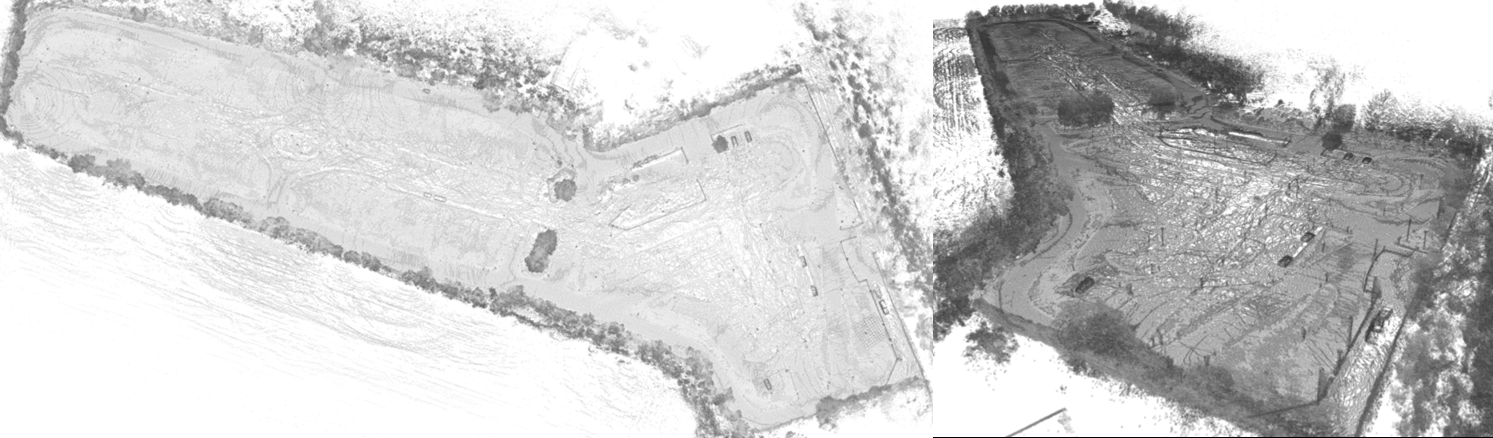
\includegraphics[width=\textwidth]{gray_jeddeloh.png}
    \caption{3D map of Jeddeloh Test area which was constructed by NDT-algorithm}
    \label{fig:3D_jeddeloh}
\end{figure}

\begin{center}
\begin{figure}
\centering
\captionsetup[subfigure]{justification=centering}
\subfloat[General view of comparison between combination of EKF with NDT (red) and NDT (blue)]{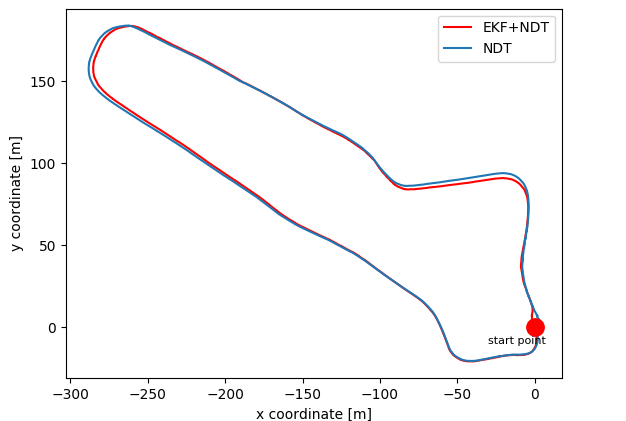
\includegraphics[scale=0.4]{jeddeloh_ekf_ndt}\label{fig:jeddeloh_ekf}}\\
\subfloat[Performance comparison between combination of EKF with NDT and NDT in 3D showed as translation and rotation error]{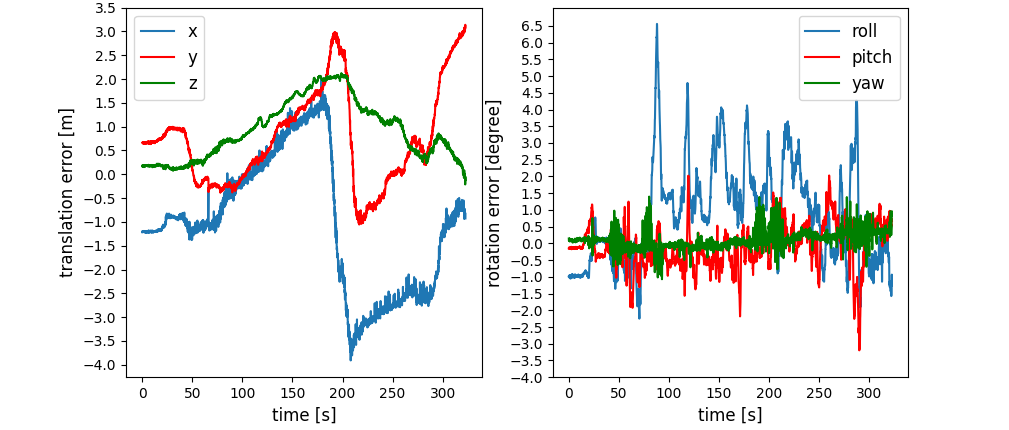
\includegraphics[height=5cm,width=\textwidth]{jeddeloh_error.png}\label{fig:jeddeloh_errorb}}
\caption{Comparison between combination of EKF with NDT and ground truth}
\label{fig:jeddeloh_error}
\end{figure}

\begin{table}
    \centering
    \small
    \begin{tabular}{|c|c|c|c|c|c|}
        \hline
         translation &max e.[m]&RMSE[m]&rotation&max e. [deg]&RMSE[deg]\\          
         \hline
         x &3.90913&1.74429& roll &6.55794&1.72251\\
         \hline
         y &3.13895&1.25324& pitch &3.19698&0.68359\\
         \hline
         z &2.19162&1.12061& yaw &1.39722& 0.30418\\
         \hline
    \end{tabular}
    \caption{Error calculation data which was subtracted from figure \ref{fig:jeddeloh_errorb}}
    \label{tab:jeddeloh}
\end{table} 
\end{center}

\newpage
\subsection{Bassum Go-kart race track Test} \label{sub:Bassum} The final test was conducted in the Bassum go-kart place and the localization algorithm was tested while the vehicle was autonomously driven.

\begin{figure}[H]
    \centering
    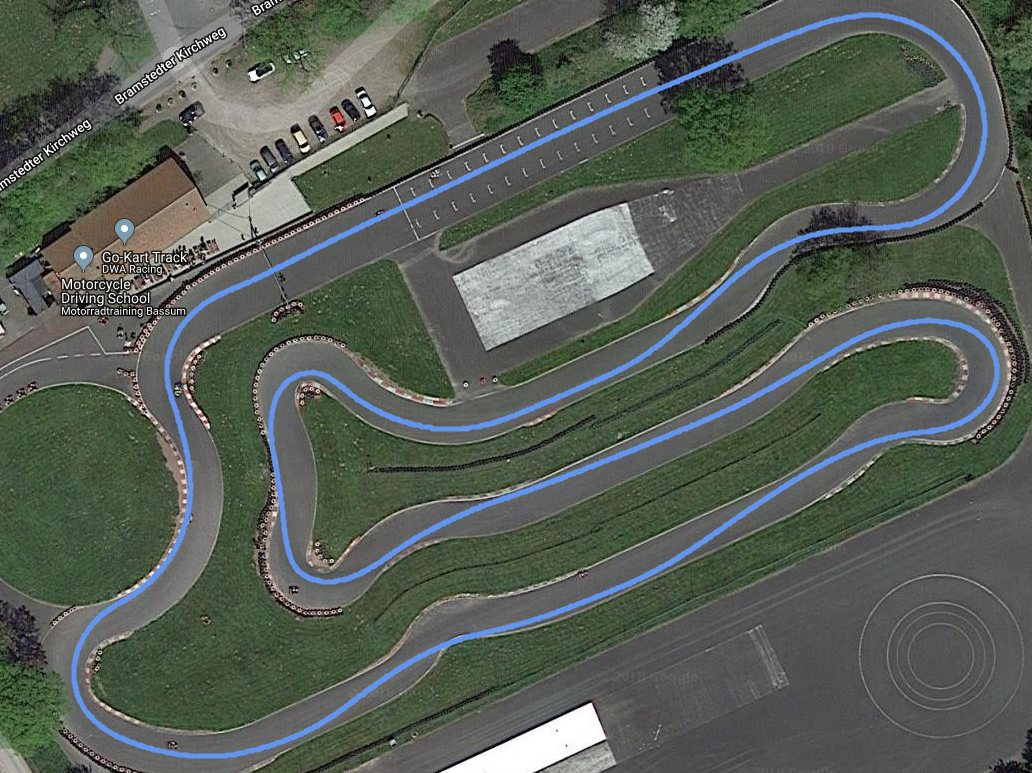
\includegraphics[scale=0.32]{bassum_gps}
    \caption{The bird view of the third test area. The vehicle was driven autonomously on the blue line which indicates the trajectory}
    \label{fig:bassum_gps}
\end{figure}
\noindent\textbf{Assessment of the Idea:} Since the real trajectory has no information about height, roll, and pitch, the evaluation was done by comparing only translation error in 2D x,y and rotation error w.r.t z-axis between NDT and the real trajectory. On the graphs above show the result of the NDT localization algorithm under the optimal circumstance, using a map and source whose resolution 0.2m and 3m, respectively. Therefore, the maximum translation/rotational error of the algorithm smaller than 0.4 m/deg, as stated in the table \ref{tab:bassum}.
\begin{figure}[H]
    \centering
    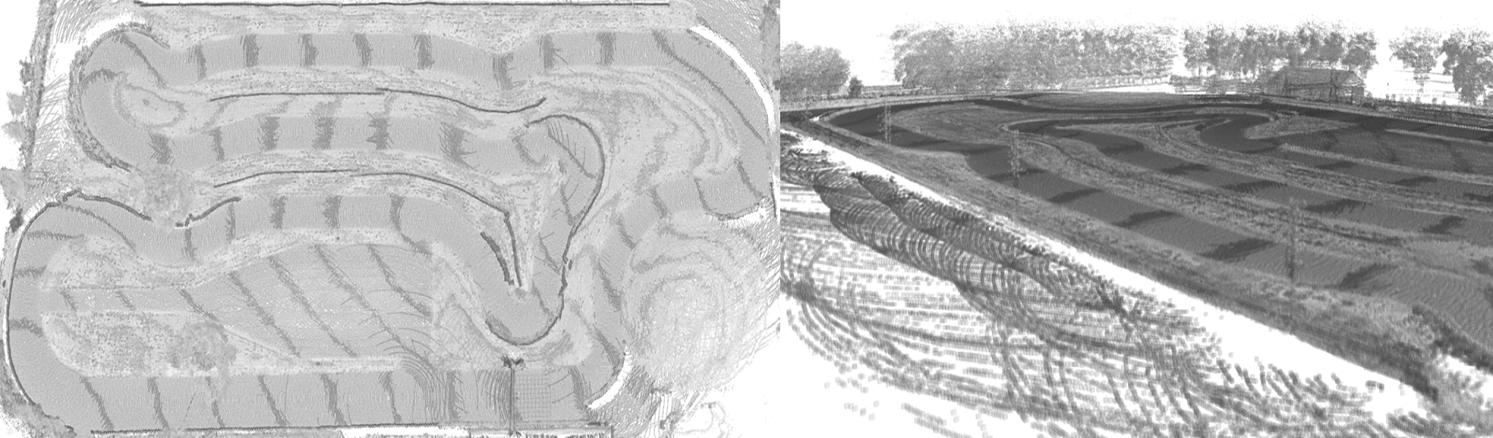
\includegraphics[width=\textwidth]{gray_bassum.png}
    \caption{3D map of Bassum Test area which was constructed by NDT-algorithm}
    \label{fig:3D_bassum}
\end{figure}

\begin{figure}[H]
    \centering
    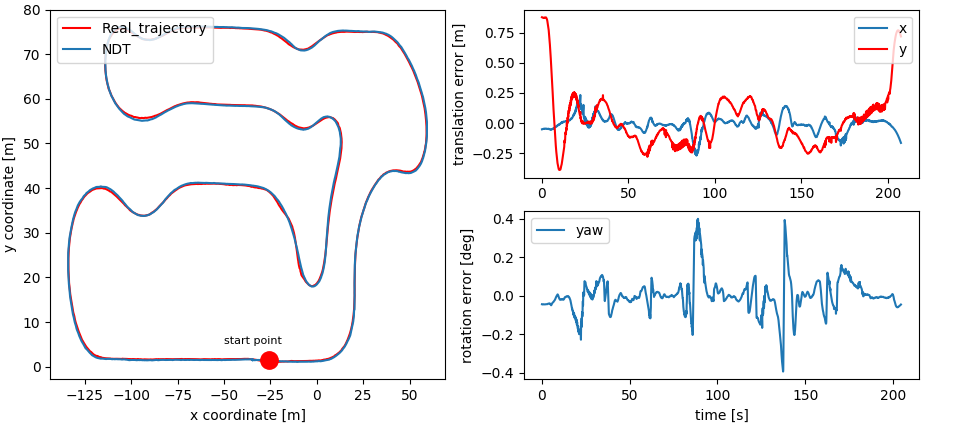
\includegraphics[height=5cm,width=\textwidth]{bassum_overall}
    \caption{NDT localization performance was shown against reference(real) trajectory comparing with translation and rotation error }
    \label{fig:bassum_overall}
\end{figure}
\vspace{-10pt}
\begin{table}[H]
    \centering
    \small
    \begin{tabular}{|c|c|c|c|c|c|}
        \hline
         translation &max e.[m]&RMSE[m]&rotation&max e. [deg]&RMSE[deg]\\  
         \hline
         x &0.21895&0.00184 & roll &-& -\\
         \hline
         y &0.37582&0.01251 & pitch & -& -\\
         \hline
         z &-&- &yaw &0.35267& 0.00118\\
         \hline
    \end{tabular}
    \caption{Error calculation data which was subtracted from figure \ref{fig:bassum_overall}}
    \label{tab:bassum}
\end{table}

\newpage
\section{KITTI Dataset}\label{sec:KITTI-set}
This section was conducted by \acrfull{kitti} data set, which is provided by KITTI. It was used to verify the results of our localization algorithms. Even though the KITTI data of interest is visual odometry, optical flow and etc., provided data set is showing similarity with our data set in terms of used sensors such as IMU, GPS, LIDAR, RGB and gray cameras except only for wheel odometry. Therefore, the KITTI dataset was utilized to compare the outputs of the localization methods with KITTI ground truth that is provided by D-GPS. In following, we presented the result of the combination of EKF with NDT by using sequence number 10 KITTI data which is shown in figure \ref{fig:kitti_gps}.

\begin{figure}[H]
    \centering
    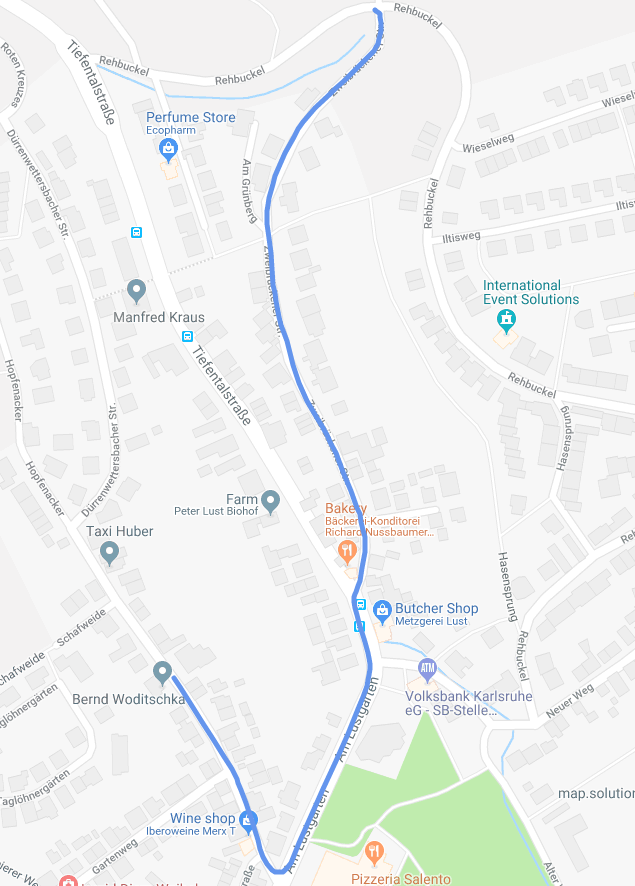
\includegraphics[scale=0.40,angle=90]{kitti_gps}
    \caption{The bird view of the KITTI test area. GPS trace was indicated blue line}
    \label{fig:kitti_gps}
\end{figure}
\noindent \textbf{Assessment of the Idea:} Since our aim is making an objective comparison, we benefit KITTI data and like in previous examples, we carried out same experiments and presented in figures \ref{fig:kitti_ndt}-\ref{fig:kitti_overall} and table \ref{tab:kitti_ndt}-\ref{tab:kitti}.
\par We, first, tested NDT algorithm with KITTI and observed that the behavior of obtained result almost the same as the previous example but with a slight difference. We assumed that the reason would be is the travelling velocity during the test drive, since our average speed was 10 km/h whereas their average speed was 20km/h. As a conclusion, we realized that after exceeding a certain limit of speed, it would cause discontinuity on localization. We also tested the other two methods ICP and combination of EKF with NDT and observed same behaviors once again. However, testing the EKF method was difficult than the previous example due to absence of wheel odometry so we could not thoroughly test EKF. Nevertheless, we presented its results even though its result was not satisfying.  
\par As a conclusion, we showed that NDT algorithm was the most successful methods among the other according to run different tests.
\begin{figure}[t]
    \centering
    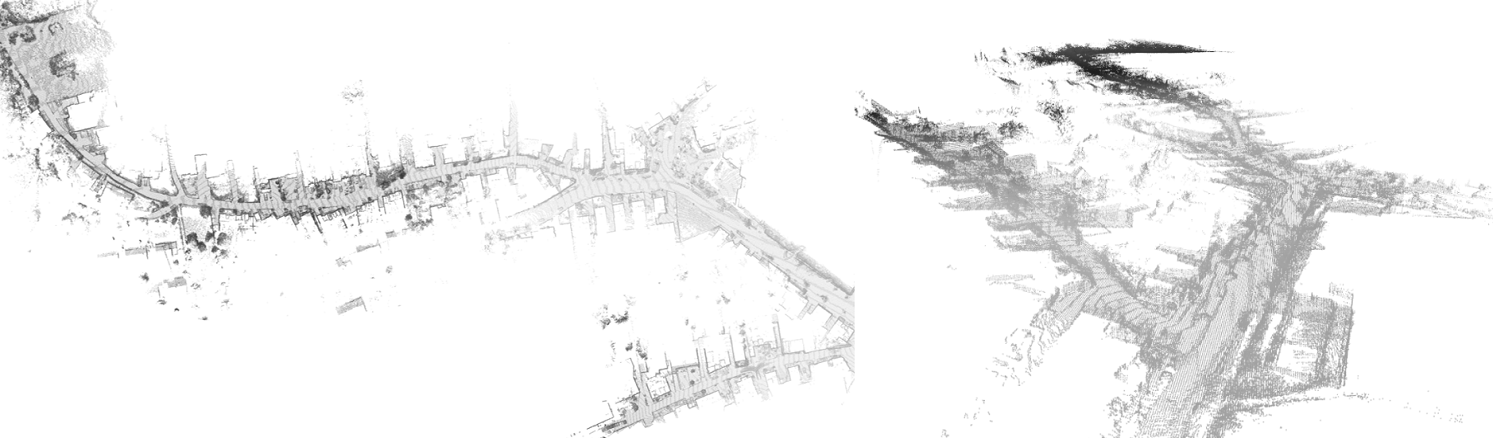
\includegraphics[height=7cm,width=\textwidth]{gray_kitti.png}
    \caption{3D map of KITTI sequence 10th test area which was constructed by NDT-algorithm}
    \label{fig:3D_kitti}
\end{figure}
\begin{figure}[H]
    \centering
    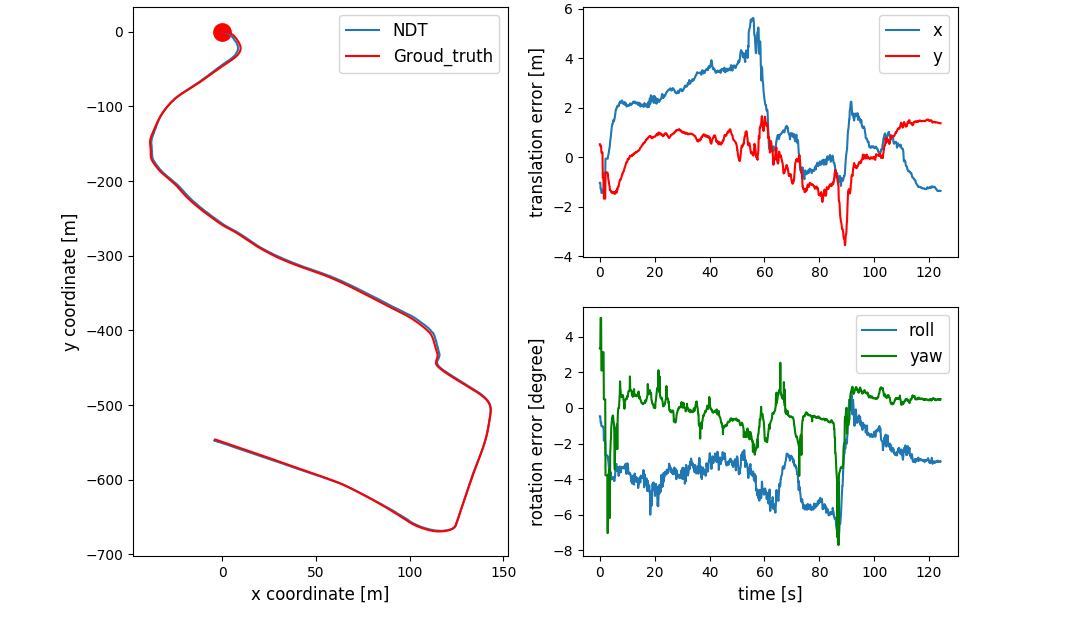
\includegraphics[height=7cm,width=\textwidth]{kitti_ndt_overall}
    \caption{Comparison between NDT and KITTI ground truth}
    \label{fig:kitti_ndt}
\end{figure}
\vspace{-0.5cm}
\begin{table}[H]
    \centering
    \small
    \begin{tabular}{|c|c|c|c|c|c|}
        \hline
         translation &max e.[m]&RMSE[m]&rotation&max e. [deg]&RMSE[deg]\\ 
         \hline
         x &5.63079  &2.24201   & roll   &-& -\\
         \hline
         y & 3.54759    &1.02374& pitch  & -& -\\
         \hline
         z &-          &-       &yaw& 7.71277 & 1.19939\\
         \hline
    \end{tabular}
    \caption{Error calculation data which was subtracted from figure \ref{fig:kitti_ndt}}
    \label{tab:kitti_ndt}
\end{table}

\begin{figure}[H]
    \centering
    \includegraphics[height=7cm,width=\textwidth]{kitti_icp_overall}
    \caption{Comparison between ICP and KITTI ground truth}
    \label{fig:kitti_icp}
\end{figure}
\vspace{-0.5cm}
\begin{table}[H]
    \centering
    \small
    \begin{tabular}{|c|c|c|c|c|c|}
        \hline
         translation &max e.[m]&RMSE[m]&rotation&max e. [deg]&RMSE[deg]\\ 
         \hline
         x &14.0997  &3.36805   & roll   &-& -\\
         \hline
         y &26.42694    &3.14686 & pitch  & -& -\\
         \hline
         z &-          &- &yaw& 41.34196 &9.19015\\
         \hline
    \end{tabular}
    \caption{Error calculation data which was subtracted from figure \ref{fig:kitti_icp}}
    \label{tab:kitti_icp}
\end{table}

\begin{figure}[H]
    \centering
    \includegraphics[height=6cm,width=\textwidth]{kitti_ekf_overall}
    \caption{Comparison between the combination of EKF with NDT and KITTI ground truth}
    \label{fig:kitti_overall}
\end{figure}
\vspace{-0.5cm}
\begin{table}[H]
    \centering
    \small
    \begin{tabular}{|c|c|c|c|c|c|}
        \hline
         translation &max e.[m]&mean e.[m]&rotation&max e. [deg]&mean e.[deg]\\ 
         \hline
         x &11.54453   &-0.88060  & roll   &-& -\\
         \hline
         y &6.82168    &-0.60853 & pitch  & -& -\\
         \hline
         z &-          &-       &yaw& 2.27149 & -0.67337\\
         \hline
    \end{tabular}
    \caption{Error calculation data which was subtracted from figure \ref{fig:kitti_overall}}
    \label{tab:kitti}
\end{table}

\section{Discussion}
Within the context of this thesis, several tests were performed and their results were presented in this chapter. However, there are some points need to be justified and discussed. We, here, would like to drag the attention of readers to these points. We expect that the combination of the EKF with NDT algorithm return more precise and smooth result. However, as shown in example \ref{sub:Bassum}, its result was somehow shifted to the right side of the ground truth. We believe that there are some reasons which cause this problem.  
\par The first reason would be a 3D map creation. Due to the inherent noise from LIDAR sensor, the accuracy of the map was not as perfect as ground truth. Therefore, it might cause a slight difference between the derived pose of the vehicle from scan matching methods and ground truth.
\par The second reason would be the absence of wheel odometry especially in case of KITTI data. Since there is no connection between the map and odometry which is explain in more detail in  REP-105\footnote{\url{http://www.ros.org/reps/rep-0105.html}}(conventions and semantic meaning for coordinate frames of mobile platforms used with ROS), it causes discontinuity, thus, EKF output had a discrete jump in order to converge true estimation.
\par Apart from these, in order to get a smoother result from these two scan matching algorithm, we would reduce the size of the voxel filter, by doing so, we would increase the overlap area and therefore, the estimated pose error decreases correspondingly the voxel size.


%----------------------------------------------------------------%
%-------------------------------CHAPTER6-------------------------%
\chapter{Conclusion}
\section{Discussion}\label{sec:discussion}
\newpage
\section{Future Work}


\appendix
\chapter{Hardware and software architecture}
In this appendix, a brief overview of our vehicle's hardware and software, which are used for the sake of this thesis, are provided.
\section{Vehicle Hardware}
In CERMcity project, MIA is a 2011 French electric car used. It features an electronically actuated throttle, brake, and steering system. To enable self-driving ability, the following sensors on our vehicle are deployed:
\begin{itemize}
    \item A Mobileye camera is image Processing Chip provides high-performance real-time image processing with vehicle and pedestrian detection in range of 150m and 40m, respectively. See fig. \ref{fig:mobileye}
    \item A ibeo Wide Angle Scanning (ScaLa) is a 145-degree field of view, a horizontal angular resolution of 0.25 degrees, and a 25Hz spin rate. See fig. \ref{fig:scala}
    \item A Delpi ESR multimode Electronically Scanning RADAR sensors with a range of 175m and a 45-degree opening angle. See fig. \ref{fig:delhi}
    \item A XSens-IMU MTi-G-700 is IMU/GPS system which is consist of accelerometer, gyroscope and magnetometer with 200 Hz output. See fig. \ref{fig:mti-imu}
    \item A Velodyne HDL-32E is \acrfull{lidar} with 32 beams, a 360-degree field of view, and a 10Hz spin rate. See fig. \ref{fig:hdl32}
\end{itemize}
\vspace{-0.7cm}
\begin{figure}[H]
    \centering
    \subfloat[]{\includegraphics[scale=0.3]{mobileye}\label{fig:mobileye}}\hfill
    \subfloat[]{\includegraphics[scale=0.2]{SCALA_product_edit}\label{fig:scala}}\hfill
    \subfloat[]{\includegraphics[scale=0.2]{delphi_esr_v2_300}\label{fig:delhi}}\\
    \subfloat[]{\includegraphics[scale=0.2]{MTi-100_productimg}\label{fig:mti-imu}}
    \hspace{2cm}
    \subfloat[]{\includegraphics[scale=0.15]{HDL32E-for-web}\label{fig:hdl32}}
    \caption{Mia senses the environment with camera(a), lidar(b,e), radar(c) and imu-gps(d)  }
\end{figure}
\section{Vehicle Software}
In this section, we briefly explained what \acrshort{ros}. ROS is such an open-source operating system for robots that allows to run various executables in parallel and they are able to exchange their data and communicate between each other using a publish/subscribe messaging model.
ROS has three levels of concept but here we only discuss ROS Computation Graph Level and its basic concept including nodes, master, topics, and messages which are tools merely used in this project. We need these tools since communication is required between other subprojects’ nodes. These are the places which are performing the computation. For instance, one node can perform video stabilization, one can run extraction of railroad algorithm and another one can perform object detection then, publish their output. Moreover, a node can not only publish processing data but also can subscribe needed data from another node at the same time via a message which is a simple the data structure of ROS. By passing the message, allows nodes communicate with each other. The message can be thought as a bridge between nodes to provide an information flow. To access the information in the message, nodes use topics which navigate messages. The topic is used to determine the subject of the message. It means that one node publishes its data via message with a certain topic. One another node that is searching for particular data can acquire them with a specific topic as a subscriber. The roll of topic is to distinguish the information came from across nodes to prevent the wrong usage of information, because as mentioned before one node can publish and subscribe multi- message at the same time. Meanwhile, the topics allow nodes send or receive the message as long as they have appropriate topics. All these communication services are conducted by a master. The master allows ROS pieces to find and talk with each other.

\printbibliography[ heading=bibintoc, title={Bibliography}]


\end{document}